\documentclass[12pt]{article}

% TEMPLATE DEFAULT PACKAGES
\usepackage{amssymb,amsmath,amsfonts,eurosym,geometry,ulem,graphicx,color,setspace,sectsty,comment,natbib,pdflscape,array,adjustbox}

% ADDED PACKAGES FOR THIS MANUSCRIPT
\usepackage{palatino,newtxmath,multirow,titlesec,threeparttable,tabu,booktabs,titlesec,threeparttable,mathtools,bm,bbm,subcaption,pdflscape,tcolorbox,mathrsfs}
% endfloat,

\usepackage{afterpage}
\usepackage[hyphens]{url}
\usepackage[margin=1cm]{caption}

\usepackage[draft]{hyperref}
\newcommand{\tim}{$\,\times\,$}
% FIGURES & TABLES CAPTION STYLING
\captionsetup[figure]{labelfont={bf},name={Figure},labelsep=period}
\captionsetup[table]{labelfont={bf},name={Table},labelsep=period}

% SECTION TITLE SETTINGS
\titlelabel{\thetitle.\enskip}
\titleformat*{\section}{\large\bfseries}
\titleformat*{\subsection}{\normalsize\bfseries}

% COLUMN TYPES
\newcolumntype{L}[1]{>{\raggedright\let\newline\\\arraybackslash\hspace{0pt}}m{#1}}
\newcolumntype{C}{>{\centering\arraybackslash}p{5.2em}}
\newcolumntype{D}{>{\centering\arraybackslash}p{5em}}
\newcolumntype{R}[1]{>{\raggedleft\let\newline\\\arraybackslash\hspace{0pt}}m{#1}}


% MARGINS AND SPACING
\normalem
\geometry{left=1.1in,right=1.1in,top=1.0in,bottom=1.0in}
\setlength{\parskip}{2.5pt}

% SPECIAL CELL 
\newcommand{\specialcell}[2][c]{%
	\begin{tabular}[#1]{@{}l@{}}#2\end{tabular}}

% NO INDENT ON FOOTNOTES
\usepackage[hang,flushmargin]{footmisc}

\begin{document}

\begin{titlepage} 
\title{{Subsidized Housing and Urban Development: Evidence from South Africa}\thanks{We are grateful to Andrew Foster, Daniel Bjorkegren, Matthew Turner, Jesse Shapiro, Brian Knight, and John Friedman for their feedback and advice.  We also thank Adelaide Steedley and the Centre for Affordable Housing and Finance in Africa as well as GeoTerraImage for generous research guidance and for providing data without which this project would not have been possible.  Any opinions and conclusions expressed herein are those of the authors and do not necessarily represent the views of the the Federal Trade Commission or its Commissioners.}}
\author{\\[3em] Benjamin Bradlow\thanks{Dept. of Sociology, Brown University, Providence, RI  E-mail: benjamin\textunderscore bradlow@brown.edu}\\
 Stefano Polloni\thanks{Dept. of Economics, Brown University, Providence, RI E-mail: stefano\textunderscore polloni@brown.edu}\\ 
  William Violette\thanks{Federal Trade Commission, Washington, DC. E-mail: william.j.violette@gmail.com} \\
 \\ 
  }
\vspace{30mm}
\date{\vspace{5mm}This Version: \today}
\maketitle
\begin{abstract}

	Does subsidized housing improve neighborhood quality in developing countries? We estimate economic spillovers from a large public housing program in South Africa using geocoded deeds records, remotely sensed housing density, and census data.  To identify project impacts, we compare constructed and unconstructed projects at fine geographic levels using difference-in-differences designs.  Within project footprints, housing quality improves and subsidized formal structures successfully crowd-out slums. Yet just outside of project footprints, we detect no significant changes in housing quantity, quality, or price. 

 %\\
%\vspace{0in}\\
%\textbf{Keywords:} traffic externalities; street livability; urban policy; housing market.\\
%\vspace{0in}\\
%\textbf{JEL Codes:} O18; H4; R2; R4.\\
\bigskip
\end{abstract}
\setcounter{page}{0}
\thispagestyle{empty}
\end{titlepage}
\pagebreak \newpage

\spacing{1.4}
\section{Introduction} \label{sec:introduction}

%Fitting naturally in a treatment-effects framework, 
%Policymakers motivate these projects with two central arguments.  
%with two central goals
%- put in perspective 
%35,786 mill 1 757 451 (2\%) of government budget

30\% of urban populations in the developing world live in crowded slums characterized by low infrastructure access, unsanitary conditions, and high crime rates \citep{mdg}. These living conditions are thought to pose long-lasting obstacles to upward mobility and local economic development \citep{marx2013slums}. We study a common policy response where governments replace slums with serviced formal structures and move slum dwellers into public housing projects. 

The promoted goals of these programs are twofold. First, policymakers stress how subsidized housing improves household wellbeing along a variety of dimensions. This is well supported by existing studies on direct recipient impacts, which link housing programs to improvements in child health, women's employment, and quality of life \citep{cattaneo2009housing,franklin2016enabled,galiani2017shelter}. A second set of policy goals pertains to broader urban development impacts, driven by spillovers to neighboring areas. For instance, subsidized housing in South Africa is proposed for ``leveraging growth in the economy, [...] combating crime, promoting social cohesion, [...] and utilizing housing as an instrument for the development of sustainable human settlements, in support of spatial restructuring'' \citep{bng}. 

Spillover effects may account for a significant share of the total welfare impacts of housing projects.  In the US, \cite{diamond2016wants} calculate that affordable housing in low-income areas generates substantial societal benefits on surrounding areas, often exceeding the total costs of the programs. Welfare effects may be even greater in developing settings, where preexisting slums impose negative externalities on neighboring areas. At the same time, lax building codes and weak zoning laws complicate predictions about the dominant effects at play. The effects of improved infrastructure and greater housing quality may be mitigated if demand in the informal housing market responds to these amenities. For example, \cite{Brueckner2018backyarding} document the common practice of ``backyarding'', where households rent informal dwellings erected on the same land plots as government-sponsored houses. 

Both the policy importance and theoretical ambiguity of these mechanisms motivate empirical analysis in a developing context.  Until recently, however, data limitations have largely precluded researchers from constructing granular measurements on the quantity, quality, and price of housing, both formal and informal. Using novel data sources, this paper contributes to filling this gap by identifying impacts on local neighborhoods at high spatial resolutions.   

We analyze the direct and spillover effects of a large public housing program in South Africa.  We combine administrative records for 57constructed and 60planned but unconstructed projects with spatial data on property transactions, formal and informal housing densities, and dwelling characteristics.  To measure spillovers, we implement a difference-in-differences design at varying distances from pro\-ject boundaries.  At every distance, we compare changes in outcomes for constructed projects to changes for planned but unconstructed projects. When feasible, our estimates include a third layer of differencing, comparing effects near versus far from project boundaries. In this way, we are able to net-out systematic time-varying differences between treated and control areas, absent project construction. Our econometric approach allows us to flexibly capture how spillover effects change across space.  Planned but unconstructed project areas provide useful counterfactuals since governments may select unobservably worse land plots to build subsidized housing projects.  These control areas resemble treated areas at baseline across a range of measures, including preexisting housing density.  


Within project boundaries, we find large improvements in access to services and home quality, but little net effects on total housing development. Compared to unconstructed areas, households living within projects (either in subsidized formal or informal housing) are more than 10 percentage points more likely to access flush toilets, indoor water taps, and electricity. The small net effects on total housing density mask a compositional change from informal to formal structures. We find greater densities of informal {\it backyard} dwellings, but not enough to offset steep declines in other types of informal housing. On the whole, these results suggest that subsidized housing projects provide positive local amenities through better house quality and improved infrastructure.

Outside project boundaries, and in spite of our previous findings, we fail to detect spillover effects  across our full range of outcomes.  Housing projects do not appear to stimulate additional construction of formal or informal dwellings at all distances outside project boundaries, up to 1200 meters away. Similarly, dwelling characteristics in neighboring areas remain largely the same after project construction.  Leveraging the exact timing of construction, we do not detect discrete changes in formal housing prices just after construction, though the data admit a wide range of treatment effects. Finally, we provide some evidence that housing markets anticipate projects, and find no indication of residents sorting, as measured by the composition of dwellers across space. 

Our findings suggest that neighborhood externalities play a minimal role in housing markets in developing countries.  Another interpretation is that informal backyard houses negate the positive benefits from government-sponsored homes. From a policy perspective, these results suggest that spillover effects may merit less emphasis than direct recipients effects in designing housing policy.  

Our analysis contributes to a recent literature focusing on the broader urban development impacts of housing policy in developing countries. \cite{baruah2017planning} study sites-and-services schemes implemented on the urban fringe of Tanzanian cities. Using comparable greenfields as counterfactuals, they find that initial infrastructure investments have long-term positive impacts on nearby housing quality. \cite{harari2018slum} examine the impacts of a slum upgrading program in Jakarta, Indonesia. The authors also use untreated comparable areas as counterfactuals, and find negative effects on land values and levels of formalization. Importantly, in a boundary discontinuity design, the authors note no evidence of spillovers from the program to neighboring areas. In ongoing work, \cite{gechter2018slums} study spillovers from formal housing development using sharp temporal changes in Mumbai's zoning laws. Through the lens of a quantitative general equilibrium model, the authors find high higher property prices,  more formal construction, and lower population density in the vicinity of targeted areas. Finally, outside of the developing world, our research draws upon an established literature on housing externalities \citep{rossi2010housing,hornbeck2017creative,diamond2016wants}. 

We proceed by first providing background on the South African housing program in Section~\ref{section:background}. 
%In Section~\ref{section:model}, we develop a conceptual framework of housing supply and housing externalities to help interpret the results. 
Section~\ref{section:data} describes the data used to measure outcomes and details our approach to identifying housing projects. Section~\ref{section:methodology} lays out the estimation strategy and identifying assumptions, which we validate with descriptive evidence in section~\ref{section:descriptives}. We present spillover results for residential home prices in Section~\ref{section:resultsprices} and demographic outcomes in Section~\ref{section:resultscensus}.  Section~\ref{section:discussion} includes a discussion of our findings before providing some concluding thoughts.


\section{Subsidized Housing in South Africa} \label{section:background}

The housing projects studied in this paper were implemented as part of a large national housing subsidy scheme enacted in 1994. Though periodically revised and renamed,\footnote{Public housing in South Africa has been delivered under the {\it Reconstruction and Development Program} (RDP) starting in 1994 and subsequently by its successor, {\it Breaking New Grounds}, as of 2004.} the program has consistently sought to redress the economic and geographic legacy of apartheid by providing formal housing to low-income households. Subsidized housing efforts at the national level have focused on constructing and allocating 40m$^2$, single-story, two-room dwellings. According to government figures, upwards of 3 million housing units have been delivered nationally between 1994 and 2015.

\subsection{Planning and Delivery}

Housing projects are often located on undeveloped state-owned land although in some cases, municipalities work with private developers to purchase inexpensive, vacant private land.  Finding suitable land plots often requires policymakers to locate the projects far from city centers and economic opportunities \citep{dhsreports}.  Undeveloped land plots may contain preexisting informal settlements, which the government tries to replace with new formal houses and ensure that preexisting residents benefit from the new project houses \citep{serihistory}.

Facing substantial housing demand, the Department of Human Settlements has continued to issue grants to provincial governments to maintain yearly housing allocations \citep{dhsreports}.  While the location and size of projects are determined by provincial and municipal governments, construction is subcontracted to private developers who also act as project managers assisting in the allocation of houses to beneficiaries \citep{seriq}. Since housing projects require coordination between many stakeholders, these pro\-jects often face unanticipated delays and cancellations due to labor and land procurement issues, difficulties gaining support from local government agencies, environmental impact assessments, and inadequate bulk infrastructure provision \citep{dhsreports}.  In one example, political disagreements with local stakeholders led to the abandonment of a large project near Johannesburg \citep{protest}.  In other cases, housing projects have been delayed for upwards of 10 years \citep{dagpl}. 


\subsection{Recipients}

The National Department of Human Settlements issues guidelines for eligibility and maintains an official waiting list for eligible households.  Eligibility requires South African citizenship, no previous property ownership, being married or having financial dependents, and having a monthly household income below R3,500 \citep{seriq}.\footnote{The Gauteng Province has implemented their own waiting list since 2008 in order to exert greater control over the allocation process.}  The share of households reporting at least one member on the waiting list has remained stable at over 13\% from 2009 to 2013.\footnote{\label{GHSnote}This figure is calculated from the General Household Surveys from 2009 to 2013}  Before construction, each project is assigned beneficiaries in a first-come, first-served basis according to the waiting list in their province or municipality. However, when projects replace existing informal settlements, previous inhabitants receive renovated houses while remaining units are allocated according to the housing waiting list.

In practice, these guidelines are loosely followed.  Recent reports point to cases of corruption in the allocation of houses while in some instances, housing projects are organized with the assistance of local community groups who ultimately select the beneficiaries \citep{seriq,casestudytinazonke}.  Research suggests that beneficiaries are often selected over the course of project construction and sometimes even after construction has finished \citep{seriq}. Beneficiaries are expected to pay a small one-time payment in order to receive title for their houses.  Guidelines also prevent beneficiaries from reselling their houses within their first 7 years of ownership.  Despite these guidelines, only 82\% of project houses are reported as being still occupied by their original beneficiaries within five years of construction.\textsuperscript{\ref{GHSnote}} Anecdotal evidence suggests that project managers are aware of active secondary markets but have difficulty policing these transactions \citep{resale}.

\subsection{Backyard Shacks}

By design, subsidized housing in South Africa offers recipients generous amounts of yard space, often diverted to alternative land uses. The construction of informal backyard shacks is a common occurrence within project boundaries. Recipients typically enter agreements with tenants (at times relatives) to lease the shacks for cash or in-kind payments. According to the 2011 census, backyard tenants represent 7.5\% of South African households.\footnote{This figure jumps to 12.5\% for the province of Gauteng, where our study is conducted.} Though the structures are not as durable as their government-provisioned counterparts, living conditions are typically superior to conventional informal settlements. Tenants gain indirect access to their landlord's services such as water taps, electricity connections, and toilets, and benefit from reduced eviction threats and greater personal safety \citep{beall2003social}. \cite{Brueckner2018backyarding} note that {\it backyarding} is suggestive of inefficiencies in the program delivery, and allows to correct potential misallocations of resources. Importantly for our analysis, backyard shacks reveal that more households may benefit from subsidized housing than the listed number of direct recipients. According to the General Household Surveys (2009-2013), more than 33\% of government-provisioned homes have backyard shacks within two years of the delivery date. 

%\section{Conceptual Framework}\label{section:model}
%Stay tuned.

\begin{comment}
We consider housing projects as generating positive shocks to housing quantity as well as quality.  Following a standard model of housing supply and demand, increases in formal housing quantity should (1) lower prices of formal housing nearby and (2) incentivize households to move into project areas, both leading to increases in population.  At the same time, gains in housing quality not only benefit direct recipients, but also may have an amenity effect, increasing the desirability of living in neighboring areas \citep{diamond2016wants}.  This amenity effect is likely to (1) increase house prices nearby and (2) drive increases in local population as well.  Taken together, quantity and quality effects have ambiguous predictions for formal housing prices nearby but both predict increases in population both within and around housing project areas.

This simple framework ignores additional features specific to housing markets in developing countries.  In the housing production function, there may be complementarities or substitution between project housing and informal housing.  By zoning and servicing large swaths of land, housing projects may lower the cost of building new informal housing settlements both within and around these projects.  At the same time, clearly defined property rights allocated by these housing projects may increase the cost of squatting, decreasing nearby informal settlements.

The level of informal settlement growth generated by these housing projects may have additional welfare consequences due to general externalities from slum growth \citep{10.1257/jep.27.4.187}.  Health effects, congested infrastructure, and higher crime combine to form negative amenities, potentially depressing nearby housing prices or lowering population densities in these areas.  Although these specific mechanisms are difficult to precisely identify in this setting, these considerations motivate analyzing the differential impacts of housing projects for informal versus formal housing.
\end{comment}

\section{Data Sources}\label{section:data}

Our analysis focuses on the South African province of Gauteng, both the smallest geographically and most populated province in the country. Gauteng's boundaries roughly correspond to the greater metropolitan areas of Johannesburg and Pretoria. Understanding the local development impacts of public housing requires (1) outcomes measured at high spatial resolutions, and (2) a precise measure of the location, timing, and size of housing projects.  To this end, we rely on four main data sources: administrative maps describing housing policies in Gauteng, deeds data on housing transactions, household-level census data, and building-based land use information. Each is described in turn below.

\subsection{Deeds Data and Location of Housing Projects}

 We locate housing projects using a combination of administrative policy maps and deeds data. We obtain the former from the Gauteng City Regional Observatory, a research unit composed of the Gauteng Provincial Government and two Johanesburg universities.\footnote{\href{url}{www.gcro.ac.za/}} The maps describe 642planned housing projects as of 2008, including notes on their completion status for some projects.\footnote{Since this data comes in the form of overlapping shapefiles, we use the union of intersecting shapes, excluding small shapes below 0.5 km$^2$.} The latter is sourced from the South African National Deeds Office, covering the 2001 to 2011 universe of transactions in {\it affordable areas}, defined as census enumeration areas with 2010 mean house prices below R500,000. These data were kindly provided by the Affordable Land and Housing Data Centre, which tracks affordable housing markets. Transaction information includes sale price, GPS location, plot size, buyer name, and seller name.

\begin{table}[h!]
\vspace{4mm}
\caption{Top-Five Sellers in Housing Transactions Sample}\label{table:topfivesellers}
\vspace{-2mm}
\centering
\begin{tabu}{lc}
\toprule
 Seller Name & Observations \\
\midrule
City Of Johannesburg Metropolitan Municipality & 29,087  \\
City Of Johannesburg & 27,672  \\
City Of Tshwane Metropolitan Municipality & 24,780  \\
Ekurhuleni Metropolitan Municipality & 21,758  \\
Gauteng Provincial Housing Advisory Board & 13,058  \\
{\bf Total Observations }& {\bf 549,704}  \\
\bottomrule
\end{tabu}

\vspace{-4mm}
\end{table}

 \subsubsection*{Constructed Housing Projects}

 Using the administrative policy maps, we define projects as successfully constructed when we observe recipients receiving deeds to their government-sponsored house within the projects' boundaries. To identify state-sponsored housing transactions, we follow a filtering procedure established by the data provider. Properties are first assumed to belong to a housing project if the seller name includes a government, municipality, or large developer when first transacted. In 	\mbox{Table \ref{table:topfivesellers}}, we show that these institutional sellers represent an important share of our sample. We then exclude deeds flagged as large buildings used for commercial purposes (less than 2\% of transactions), as well as purchase prices more than R50,000 above the yearly nominal subsidy values (less than 4\% of remaining transactions). As shown in the right panel of Figure \ref{figure:transactionhist}, transaction prices for properties deemed to belong to public housing programs exhibit significant mass-points in their distribution, consistent with many properties being recorded with these subsidy values. Finally, we exclude transactions occurring in Gauteng's historic townships, because the bulk of residential construction within these areas precedes the start of South Africa's housing program.\footnote{Urban townships are apartheid-era residential areas created for black migrant workers. Township boundaries were also provided by the Gauteng City-Region Observatory.} Altogether, this filtering procedure identifies over 127,000 properties as government-sponsored housing. Overlaying theses properties' GPS coordinates with the housing policy maps, we are able to identify 57constructed housing projects. Delivery dates for the projects are then inferred from the distribution of transactions over time. Specifically, considering transactions within each project separately, we set the modal transaction month as the delivery month for each project. Within projects, most government-sponsored properties are transacted in the same month. %This is apparent from the upper panel of figure \ref{figure:densitytime}, where monthly transaction densities for subsidized properties are plotted 36 months prior and following the modal delivery month.

\begin{figure}[t]
\caption{Transaction Price Histogram}\label{figure:transactionhist}
\centering
\tcbox[colback=white,boxrule=.35mm,boxsep=0mm]{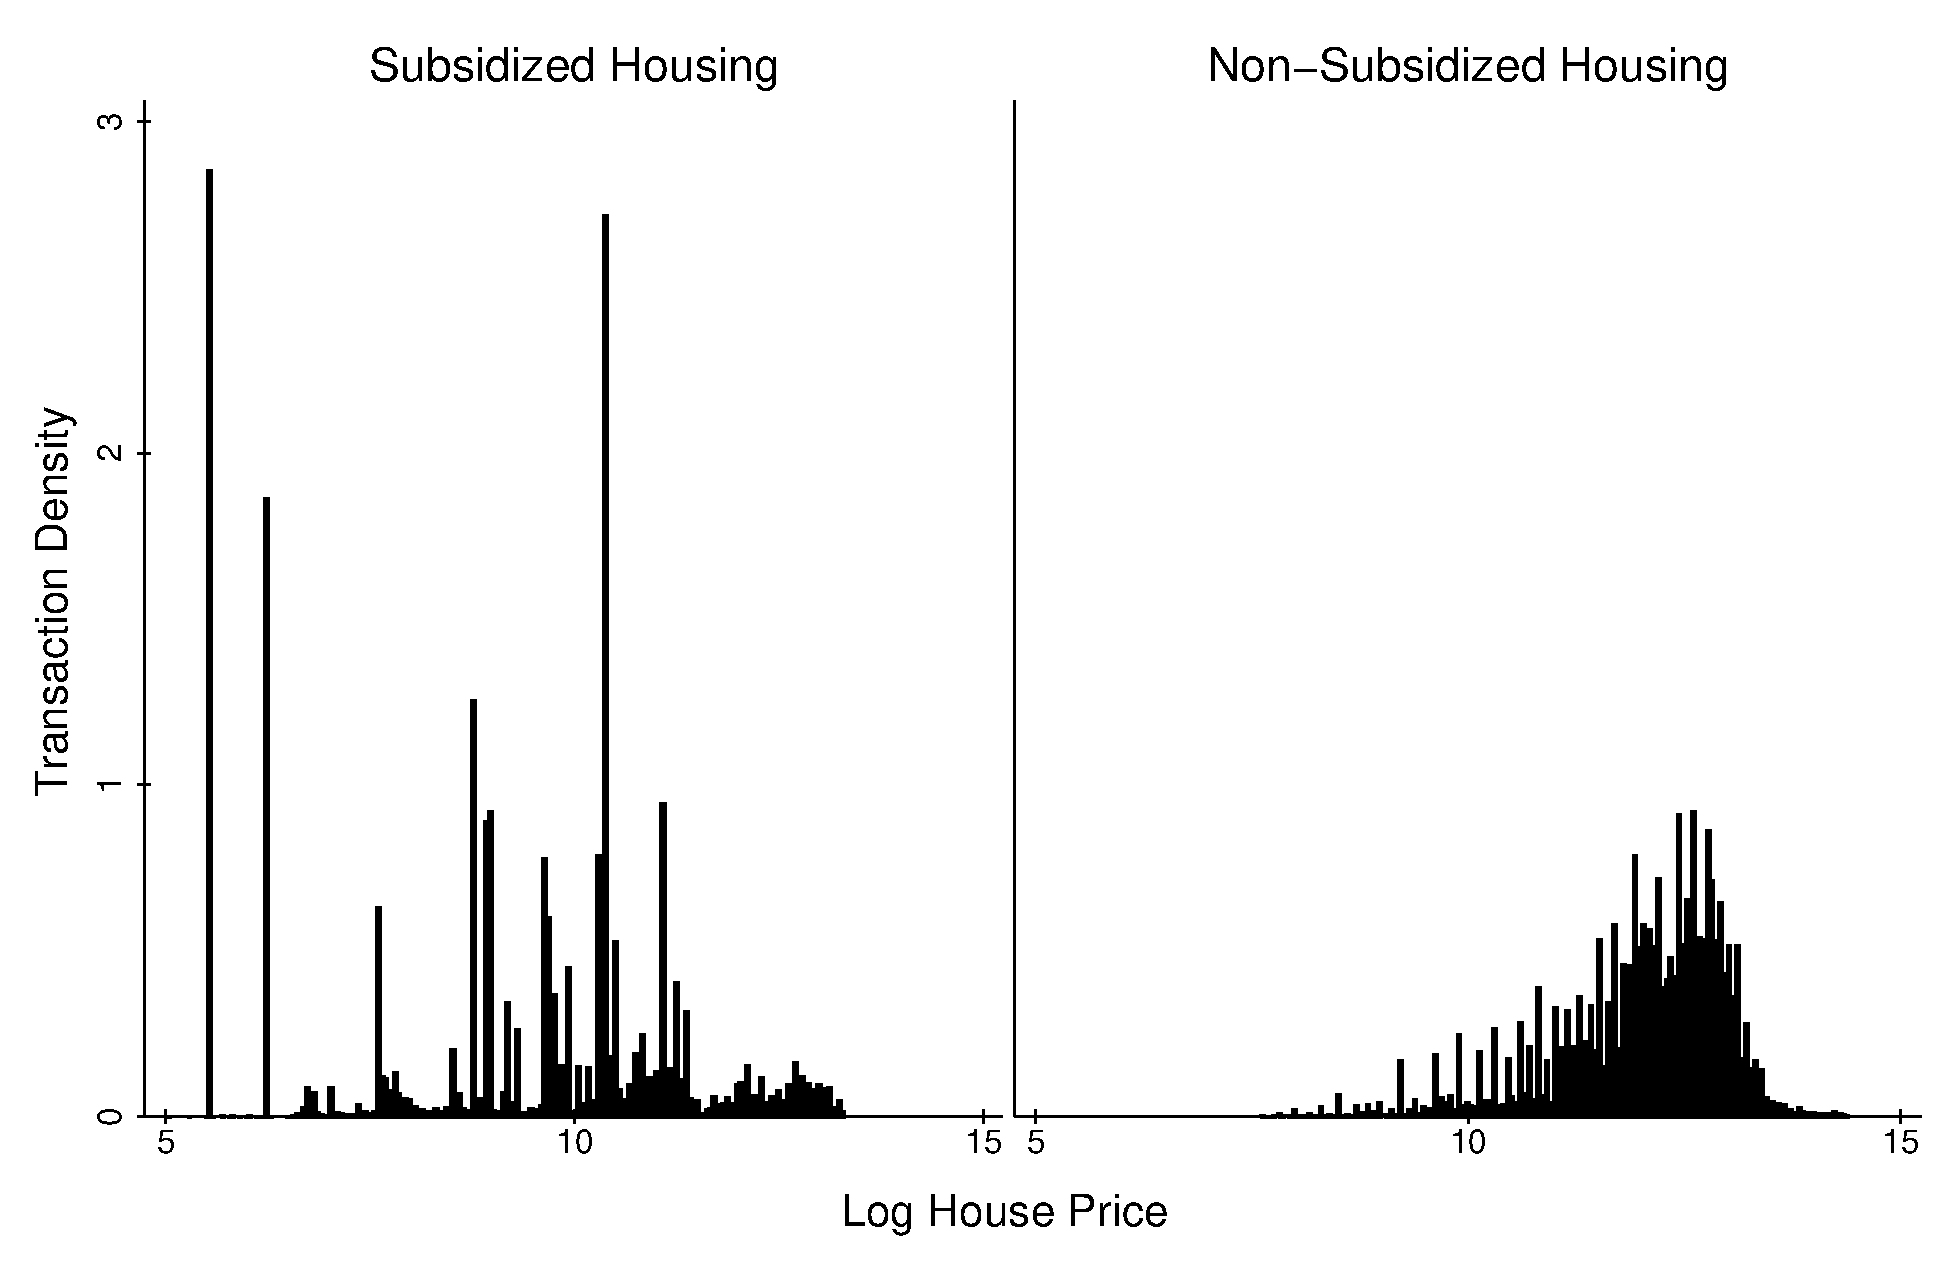
\includegraphics[scale=.4,trim={0cm 0cm -1cm 0cm}]{figures/summary_pricedist.pdf}}
%\\
%\footnotesize{Note: Transactions are censored at R100,000.}
\end{figure}

\begin{figure}[t!]
\centering
\caption{Housing Project Map}\label{figure:map}
\tcbox[colback=white,boxrule=.35mm,boxsep=0mm]{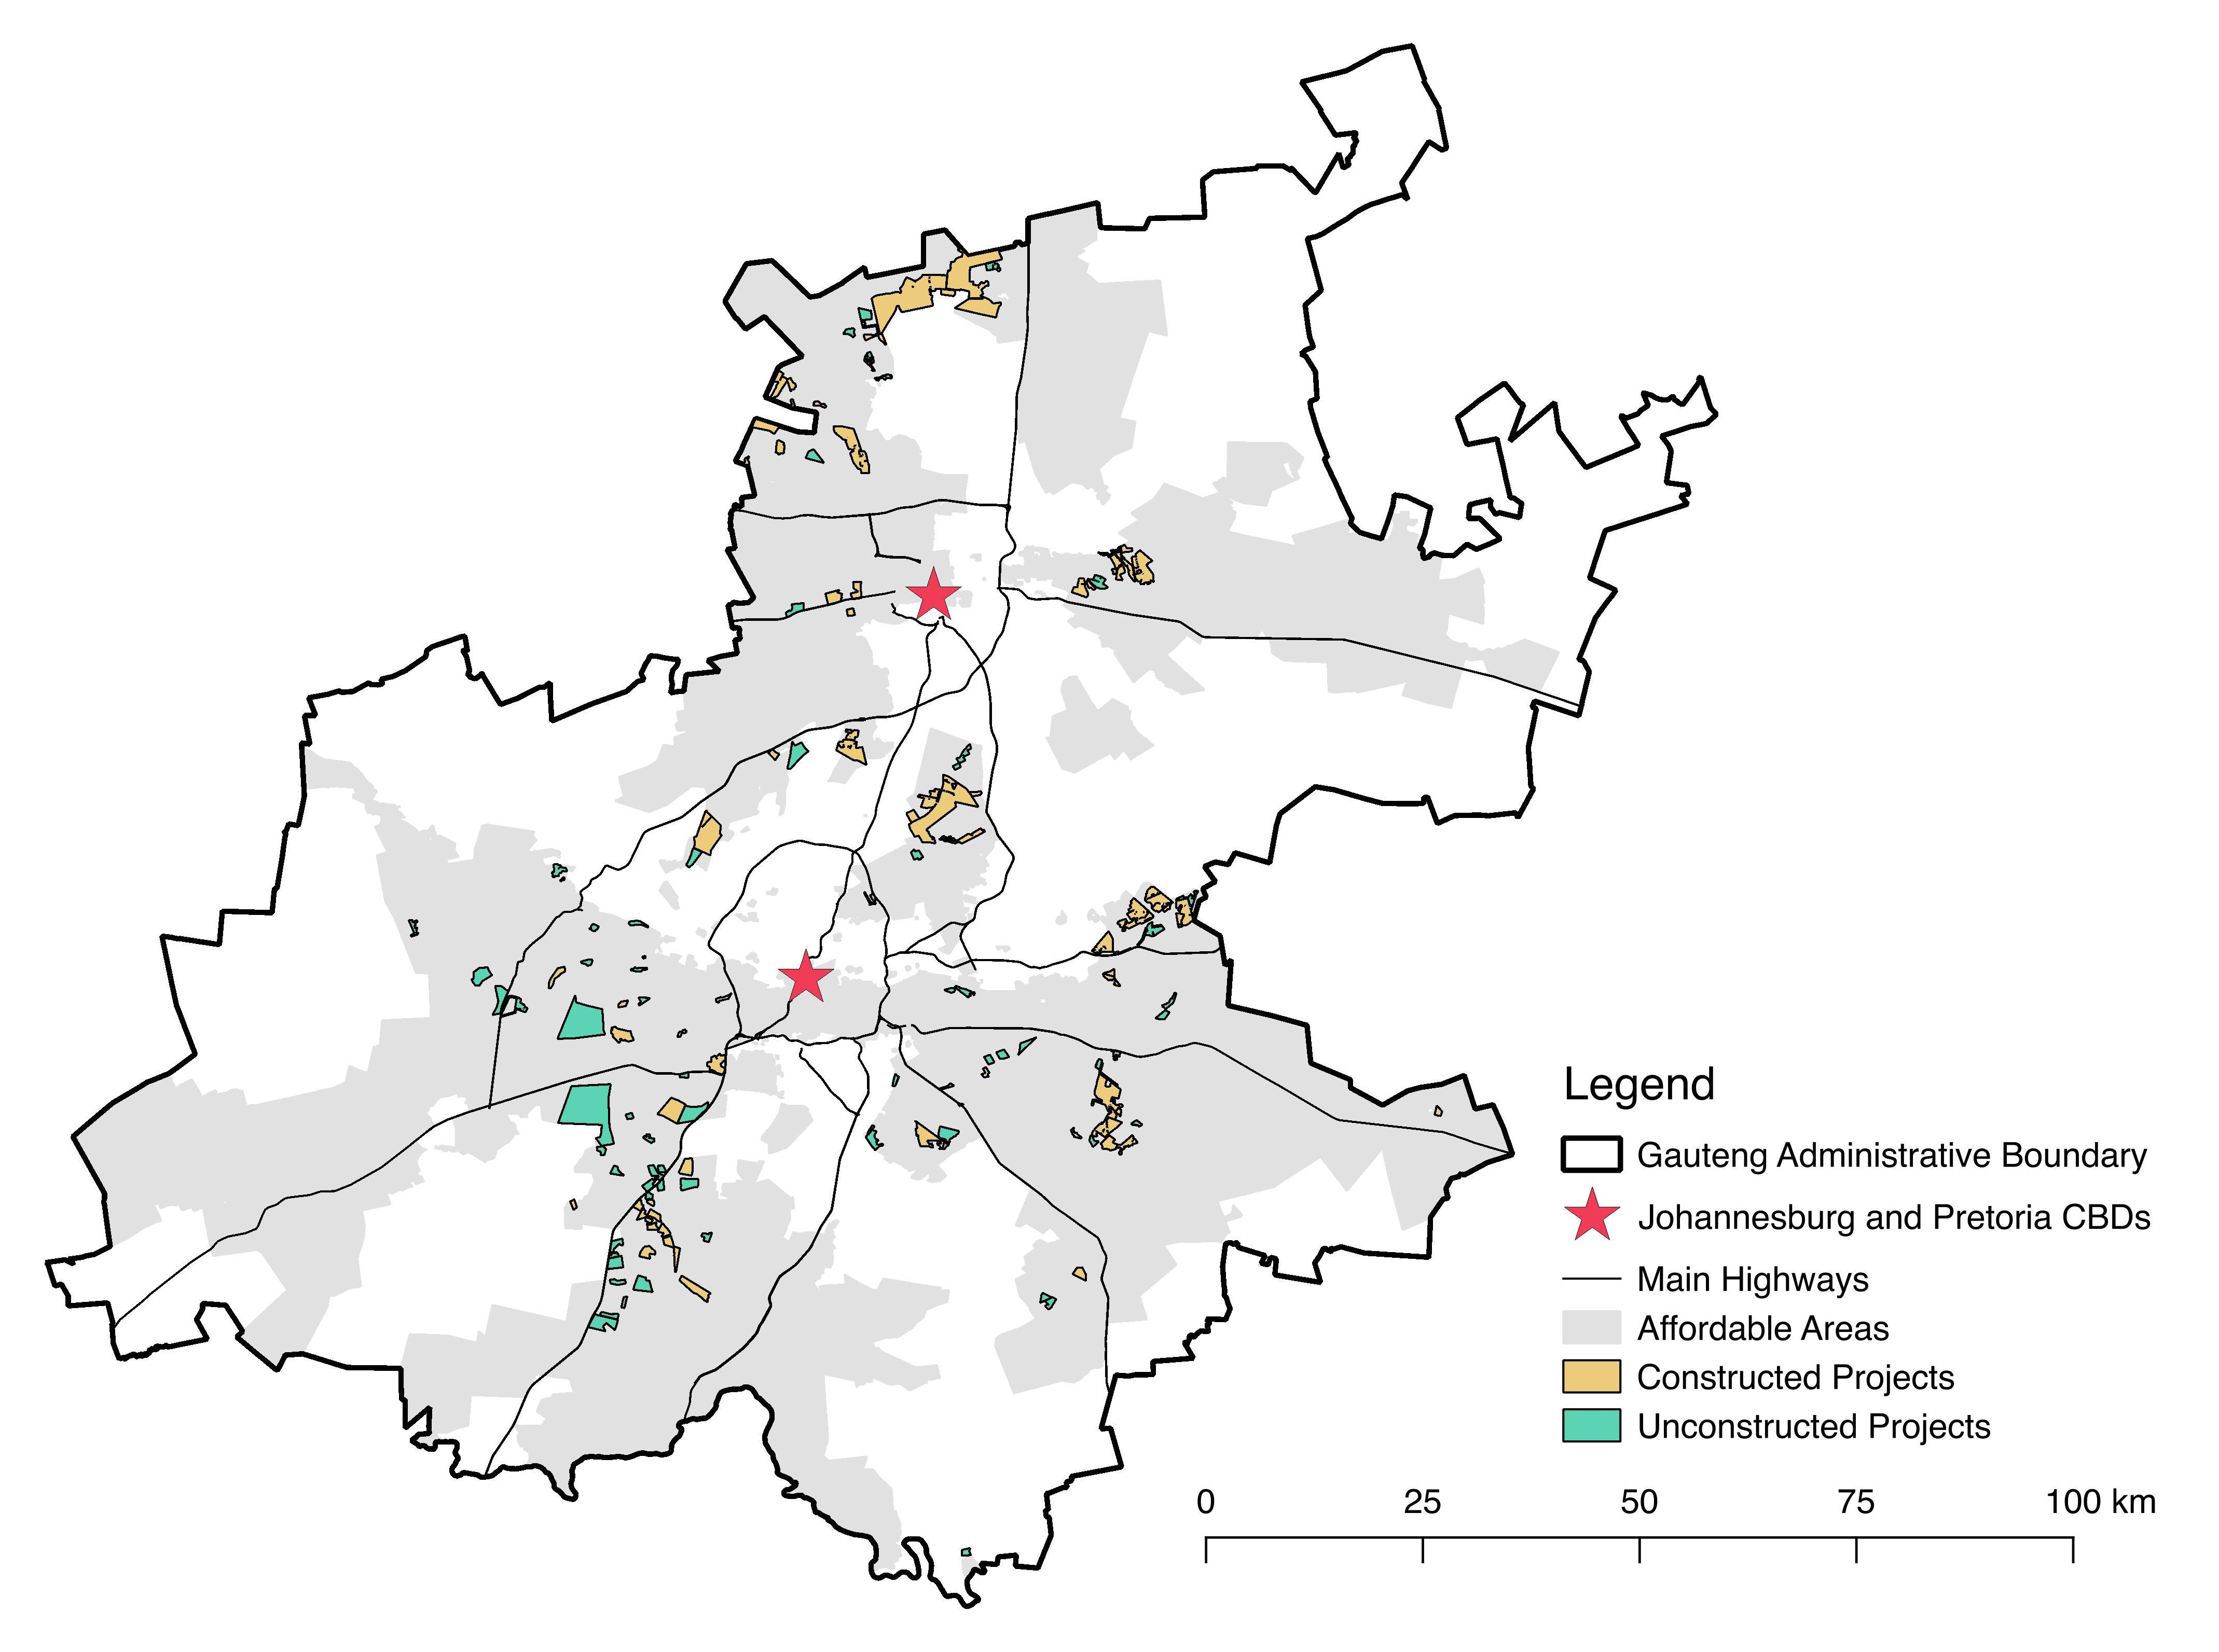
\includegraphics[scale=.098,trim={.9cm .4cm .9cm .4cm}]{figures/explanmap.jpg}}
\end{figure}

\subsubsection*{Planned but Unconstructed Housing Projects}

Identifying 57constructed housing projects leaves 99planned but possibly unconstructed housing projects in the administrative map.  We propose using these projects as counterfactuals, capturing the level of urban development that would have occurred in the absence of construction. Because our deeds data cover the 2001-2011 period and the policy maps pertain to 1994-2008, a concern is that some of the remaining 99projects were planned and delivered prior to 2001. In order to determine which of the unconstructed projects were planned between 2001 and 2011, we make use of National Treasury budget reports.  We are able to digitize data for 132 projects from budget reports spanning 2004 to 2009, which detail the name, start date, expected completion date, and cost of each housing project.  We then use a string-matching algorithm to link project names from the budget reports to the administrative maps. This procedure results in a final sample of 60unconstructed projects. We provide further details about the digitization and string-matching algorithm in Appendix~\ref{appendix:stringmatch}. For attributing construction dates to these counterfactual projects,  we use expected completion dates from the budget reports.\footnote{This will matter only for our analysis on housing prices, since we observe two time periods, pre and post, for all other data sources. }

Figure \ref{figure:map} shows the geographic setting of our analysis, displaying our final sample of constructed and unconstructed projects as polygons. Importantly, Figure \ref{figure:map} also shows that the affordable areas -- the coverage area for our deeds data -- contain every project boundary. While constructed and unconstructed projects are often adjacent to each other, possibly indicating cases where authorities were unable to complete final phases of planned projects, there are also many examples of isolated projects of both types.  Projects are generally located at relatively great distances from central business districts (CBDs), suggesting that vacant or inexpensive land plots are especially targeted by housing authorities.  Despite their distance from the CBDs, housing projects are often next to arterial highways, easing commuting costs for recipients.

\begin{table}[h!]
\centering
\caption{Project Descriptions}\label{table:projectdescriptions}
\vspace{-2mm}
\begin{tabular}{l*{1}{cc}}
\toprule
 &Constructed &Unconstructed  \\
\midrule
Proposed   &          5  &    20  \\
Planning   &          8  &    12  \\
Under Implementation& 12 &     4  \\
Complete   &          6  &     1  \\
No Description &     26  &    23  \\ 
Total             &  57  &    60  \\
\bottomrule
\end{tabular}
\end{table}

We note that our approach is not without limitations, and may introduce measurement error insofar as we are misattributing deeds to housing projects (false-positives), or wrongly assuming a project is unconstructed (false-negatives). To provide some validation for our classification, we tabulate in Table~\ref{table:projectdescriptions} project descriptions from the administrative policy maps according to whether projects are classified as constructed or unconstructed. We find that constructed projects are more likely to be classified as ``completed" or ``under implementation", while unconstructed projects are more likely to fall into ``proposed'' or ``planning'' categories.\footnote{We cannot verify that every project description, when available, is indicative of the most recent project status.} Figure \ref{fig:forchange} in section \ref{section:descriptives} further validates our sample, showing from building-based land use data (described in section \ref{section:data:bblu}) how formal housing increases disproportionately in projects classified as constructed. 


\subsubsection*{Nearby housing transactions}

To examine spillovers nearby housing projects, we include the remainder of properties that are located outside of the project areas and are not sold by government housing agencies or large developers.  We identify these developers as sellers appearing more than 30 times in the transaction sample.  Excluding these sellers limits the external validity of our results to small developers and individual homeowners.  We focus on properties located within 4 kilometers of constructed and unconstructed housing projects, forming a sample of over 140,000 transactions.  We exclude the top 1\% of prices as well as prices below 2,500 Rand, which are likely to be composed of mismeasured prices, or titles exchanged between family members. The price distribution of this sample is displayed in the right panel of Figure \ref{figure:transactionhist}, which stands in contrast to the distribution of subsidized transactions in the left panel. 

\subsection{Census Data}

To measure impacts on dwelling characteristics, we use the 2001 and 2011 National Censuses of Population and Housing. Specifically, we analyze household-level responses describing the quality of their living quarters. Our outcomes are mainly binary indicators and pertain to the household's access to services (flush toilets, water tap, electricity access), housing durability, and tenure arrangements. We identify households at the {\it small-area} level, the smallest available census geography. The province of Gauteng is divided between approximately 11,000 small areas in 2001, and 17,000 small areas in 2011.\footnote{Despite many boundaries being very similar, census geographies are not constant in both time periods. Most of the 2001-2011 growth in census small areas is due to geographies being split into more part in the 2011 census.} On average, each census area contains 170 households. Though we observe responses from every surveyed household in both census waves, the data does not allow to link households across time periods. 

\begin{figure*}[t!]
        \centering
        \caption[ Building-Based Land Use Data ]
        {\small Building-Based Land Use Data } 
        \vspace{2mm}
        \begin{subfigure}[b]{0.48\textwidth}
            \centering
            \frame{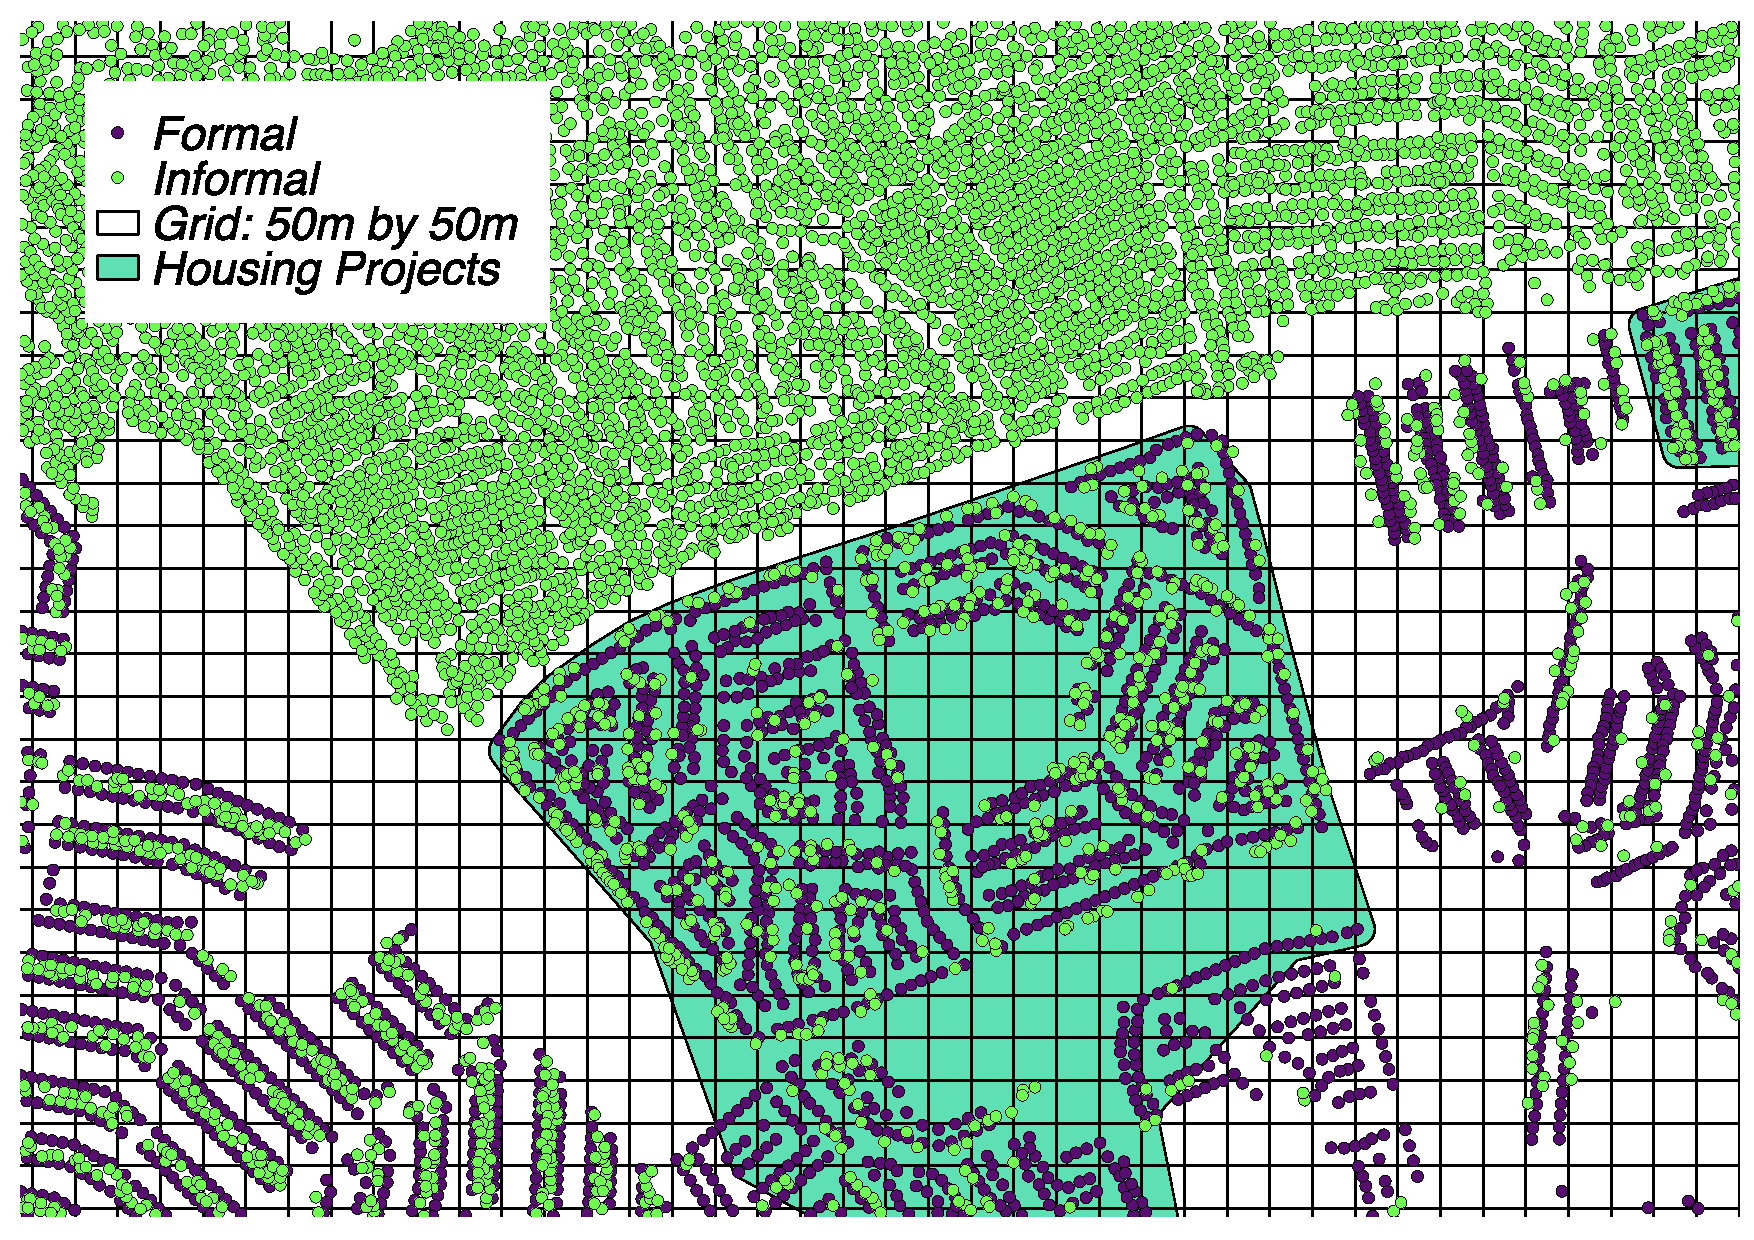
\includegraphics[width=\textwidth,trim={0cm 0cm 0cm 0cm}]{figures/bblu_map.jpg}}
            \caption[Network2]%
            {{\small raw data identifying (in)formal structures}}    
            %\label{fig:prefor}
        \end{subfigure}
        \hfill\quad
        \begin{subfigure}[b]{0.48\textwidth}  
            \centering 
            \frame{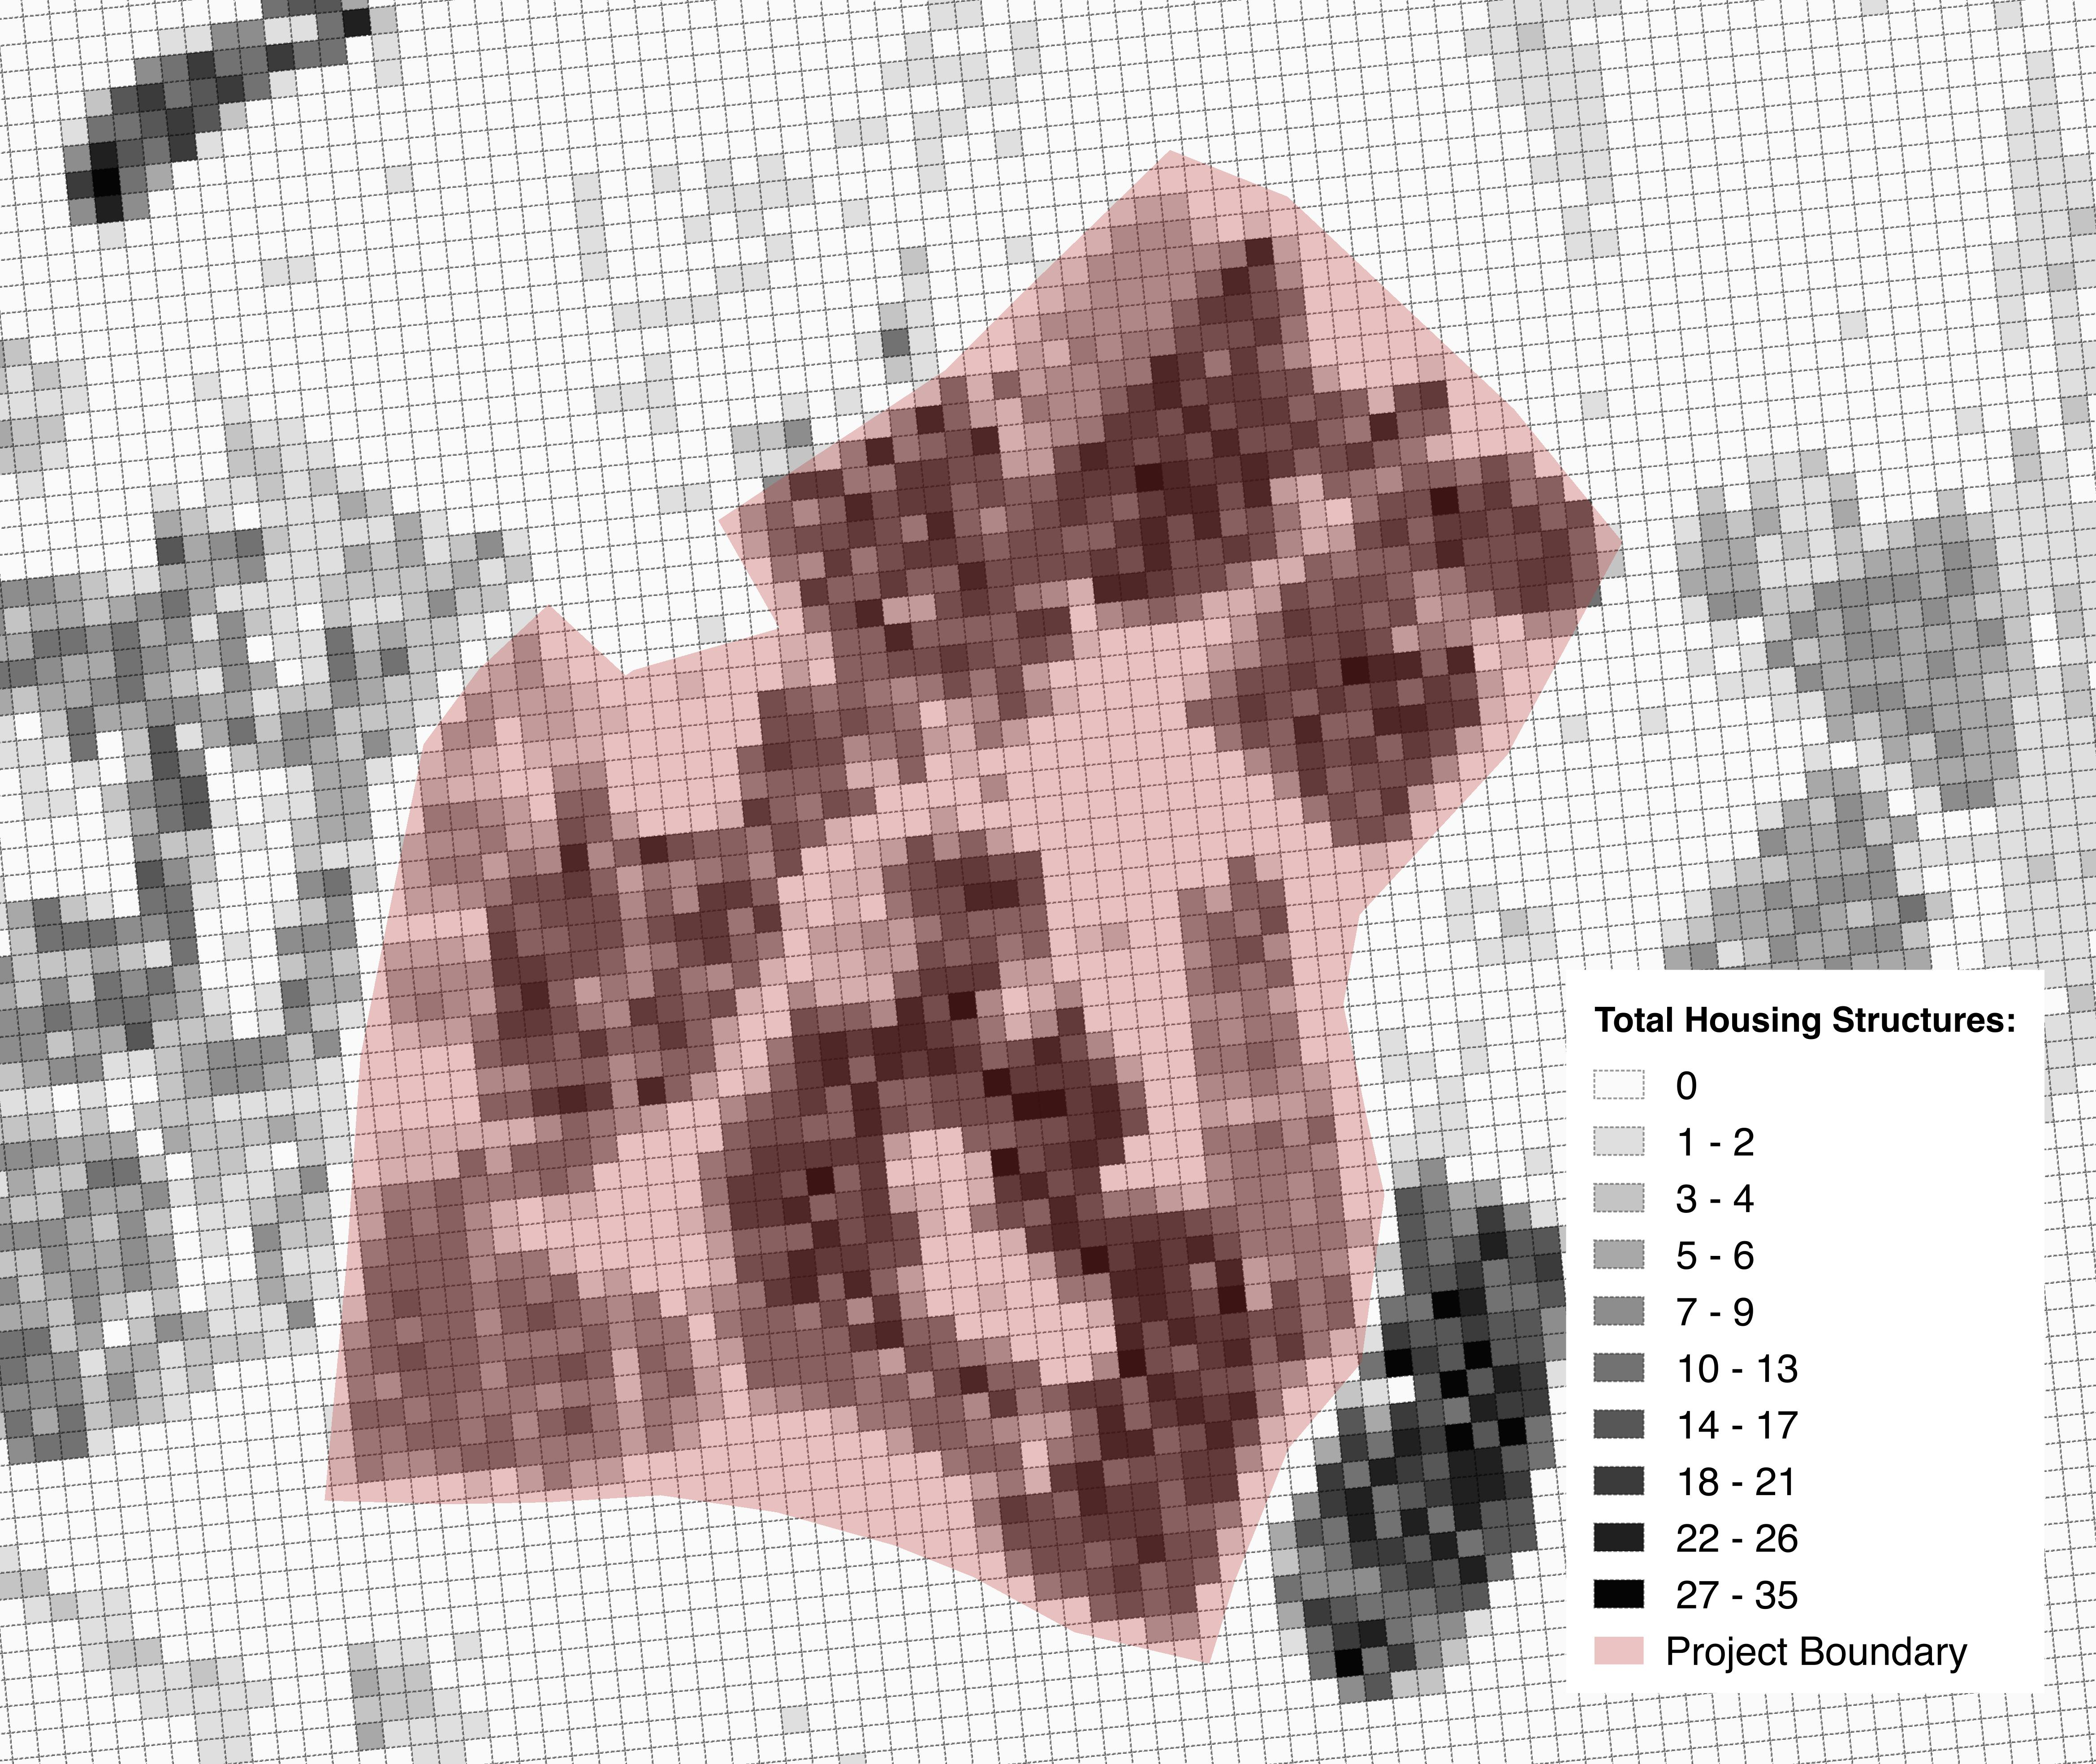
\includegraphics[width=\textwidth,trim={0cm 0cm 0cm 0cm}]{figures/bblu_grid.jpg}}
            \caption[]%
            {{\small 50m$\times$50m grid cells data aggregation}}    
            %\label{fig:preinf}
        \end{subfigure}
        \label{fig:bblumaps}
    \end{figure*} 

\subsection{Building Based Land Use}
\label{section:data:bblu}

Our final data source consists of hand-coded building surveys derived from high-resolution aerial and satellite imagery. We obtain these data from GeoTerraImage (Pty) ltd., a local remote-sensing specialist.\footnote{\href{http://www.geoterraimage.com/}{\tt http://www.geoterraimage.com/}} The data differentiates structures across over 30 categories, including formal and informal residential dwellings. Informal housing structures are easily identified from their temporary nature, often made of materials such as recycled wood and corrugated metal. In contrast, formal housing structures are permanent, generally made out of brick, and may have a pitched or a flat roof with tiles, zinc panels, or other materials. Importantly for our analysis, the data encodes backyard shacks as informal structures, but distinguishes between backyard and other types of informal buildings. We track changes in residential development by using two available survey waves in Gauteng: 2001 and 2012. As a validation exercise, we compute aggregated building counts at the census small-area level, and check the resulting figures against the number of households reporting to live in formal/informal housing in the census. The two data sources paint a consistent picture of housing in Gauteng, with high correlations ($\geq$ 0.85) between formal and informal building quantities in both available comparison years.\footnote{We correlate the 2001 and 2012 building surveys with the 2001 and 2011 censuses, respectively.} For estimation purposes, we transform this data into 50m$\times$50m grid cell aggregates, thereby creating five measures of housing density: (1) total residential structures split between (2) formal residential structures and (3) informal residential structures, which can be further decomposed into (4) backyard informal and (5) non-backyard informal structures.  These grid cells will be the main units of observations for our housing density regressions, described in section \ref{section:bbluestimates}. In Figure \ref{fig:bblumaps}, we provide an example of the raw data and a depiction of our griding procedure, using the 2012 data wave.

\section{Empirical Methodology}\label{section:methodology}

To estimate the urban development impacts of subsidized housing both within project boundaries as well as nearby, we implement a difference-in-differences strategy assessing changes in outcomes for constructed projects, using unconstructed projects as counterfactuals. Given the varying temporal and spatial resolution of our measured outcomes, we estimate different forms of the following specification:

\begin{equation}\label{eq:main}
\quad y_{ipt} \, = \, \lambda_{p} \,+\, \sum\limits_{d\in D} I^d_{ip}\Big( \alpha^d \textsc{\small Post}_{pt}\times\textsc{\small Const}_{p} \, + \, \beta^d\textsc{\small Post}_{pt} \, + \, \gamma^d\textsc{\small Const}_{p} \, + \, \theta^{d} \Big) \, + \, \delta X_{ipt} \, + \, \varepsilon_{ipt} \quad 
\end{equation}

% $D_{pt}$ and $C_{p}$ are post and treatment dummies, where 
\noindent where $y_{ipt}$ is the outcome for unit $i$ in vicinity of project $p$ observed at time $t$, with idiosyncratic error $\varepsilon_{ipt}$. $\textsc{\small Post}_{pt}$ equals one if period $t$ is after project $p$'s assigned construction date, and $\textsc{\small Const}_{p}$ equals one if project $p$ is constructed (treated). We interact the terms $\textsc{\small Post}_{pt}$, $\,\textsc{\small Const}_{p}$, and $\textsc{\small Post}_{pt}\times\textsc{\small Const}_{p}$ with a set of distance dummies $I^d_{ipt}$, where $I^d_{ipt}$ equals one if unit $i$ is located at distance $d$ from the boundary of project $p$. Our estimating equation may also include project fixed-effects $\lambda_{p}$ and a vector $X_{ipt}$ of additional controls. The set of distances $D$ partitions the land within and surrounding housing projects and varies across data sources.\footnote{$D$ is defined explicitly for every set of results in section \ref{section:results}.} This approach therefore allows for difference-in-differences estimates to vary flexibly according to the geographic exposure to housing projects.

% As will be clear from sections \ref{lol} and \ref{lol}, 
We interpret the coefficients of interest $\alpha^d$ as the causal impacts of subsidized housing on outcome $y$ at distance $d$ from a housing project. Specifically, $\alpha^d$ measures the differential change in outcomes for constructed projects, relative to unconstructed projects.  A causal interpretation requires the assumption that absent the completion of a housing project, constructed and unconstructed areas would experience the same changes in outcomes. We discuss caveats below.

By comparing unconstructed versus constructed project areas, this method builds on previous studies of housing spillovers, which instead focus on comparing areas nearby to areas just further away from projects (\cite{diamond2016wants}).  The advantage of our method is that it does not require assuming how spillover effects dissipate with distance ex-ante; instead, we directly estimate these spillovers.  It is particularly helpful to relax this assumption for evaluating South African housing programs since (1) the large sizes of projects suggest that spillover effects may extend for long distances and (2) program recipients may be drawn from wide areas around housing projects.  

A central concern for our approach is that project construction may be driven by changes in local political or economic conditions that may also affect local housing development.  For example, growing neighborhoods may generate greater political resistance to housing projects, delaying project construction despite improvements in local housing.  Alternatively, worsening infrastructure quality may both increase the costs of finishing projects while also worsening local housing conditions.  To the extent that these trends are reflected in average levels of local characteristics, we can evaluate potential sources of endogeneity by comparing baseline characteristics across constructed and unconstructed areas as in Section~\ref{section:descriptives}.  However, we are unable to test for these factors if changes in local economic and political conditions happen at the same time as project construction.

Another potential concern is that forward-looking households may anticipate investments in these areas and alter their housing investment decisions accordingly.  For example, squatter households may be more likely to construct temporary, informal structures or locate elsewhere rather than invest in long-term dwellings in these areas.  In this case, comparisons between constructed and uncontructed areas would overestimate the role of project construction in boosting formal housing development.  Similarly, nearby housing markets may anticipate projects by either appreciating or depreciating in advance (depending on the anticipated amenity value of the projects).  We are able to empirically examine these effects to some extent by closely observing dynamics in housing prices around the construction date.  For the majority of our empirical approaches, we compare changes in outcomes between 2001 and 2011 so that our baseline time-period is likely occur well before households are aware of future project construction.  This long-term comparison helps to ensure that anticipatory effects play a minimal role in biasing results.  Qualitative evidence further suggests that these effects may be limited by the substantial uncertainty in project timing due to difficulties coordinating stakeholders and sources of funding \citep{serihistory}.\footnote{\cite{diamond2016wants} also leverage uncertainty in project timing for affordable housing in the US.}

\begin{table}[b!]
\centering
\caption{Housing Projects Areas Description}\label{table:projectdescriptives}
\vspace{-2mm}
\begin{tabular}{l*{1}{cc}}
\toprule
  &Constructed &Unconstructed \\
\midrule
Number of Projects  &       57 &       60 \\
Area (km2) &       3.37 &       2.45  \\
Median Construction Year & 2005 & 2007$^*$\\
Delivered Houses  &     894.87 & .      \\
House Price within 1km (Rands$^\dagger$) &   215,172.77   &   204,490.48   \\
Distance to CBD$^\ddagger$ (km) &  31.08  &     33.43   \\
\bottomrule
\multicolumn{3}{l}{\scriptsize $^*$Calculated from {\it expected} completion dates using Gauteng National Treasury budget reports.}\\[-.5em]
\multicolumn{3}{l}{\scriptsize $^\dagger$ The USD averaged to about 7.70 Rands during the 2001-2011 period.}\\[-.5em]
\multicolumn{3}{l}{\scriptsize $^\ddagger$Measured as the average minimum distance with respect to Johannesburg and Pretoria CBDs. }
\end{tabular}
\end{table} 

\section{Descriptive Statistics}\label{section:descriptives}

%To assess the extent to which our definitions accurately measure housing projects, Figure~\ref{figure:gcrooverlap} maps our cluster definitions on top of administrative data on housing projects.  We see strong overlap between clusters and administrative projects, providing additional support for our deeds-based cluster measure.  A few smaller clusters do not overlap with administrative definitions, which is consistent with the administrative data recording larger, higher-cost projects.  Similarly, administrative boundaries that do not contain clusters are likely to be projects that were planned but were not completed or are scheduled to be completed in the future.

% \begin{figure}
% \caption{Clusters and Administrative Project Boundaries}\label{figure:gcrooverlap}
% \centering
% 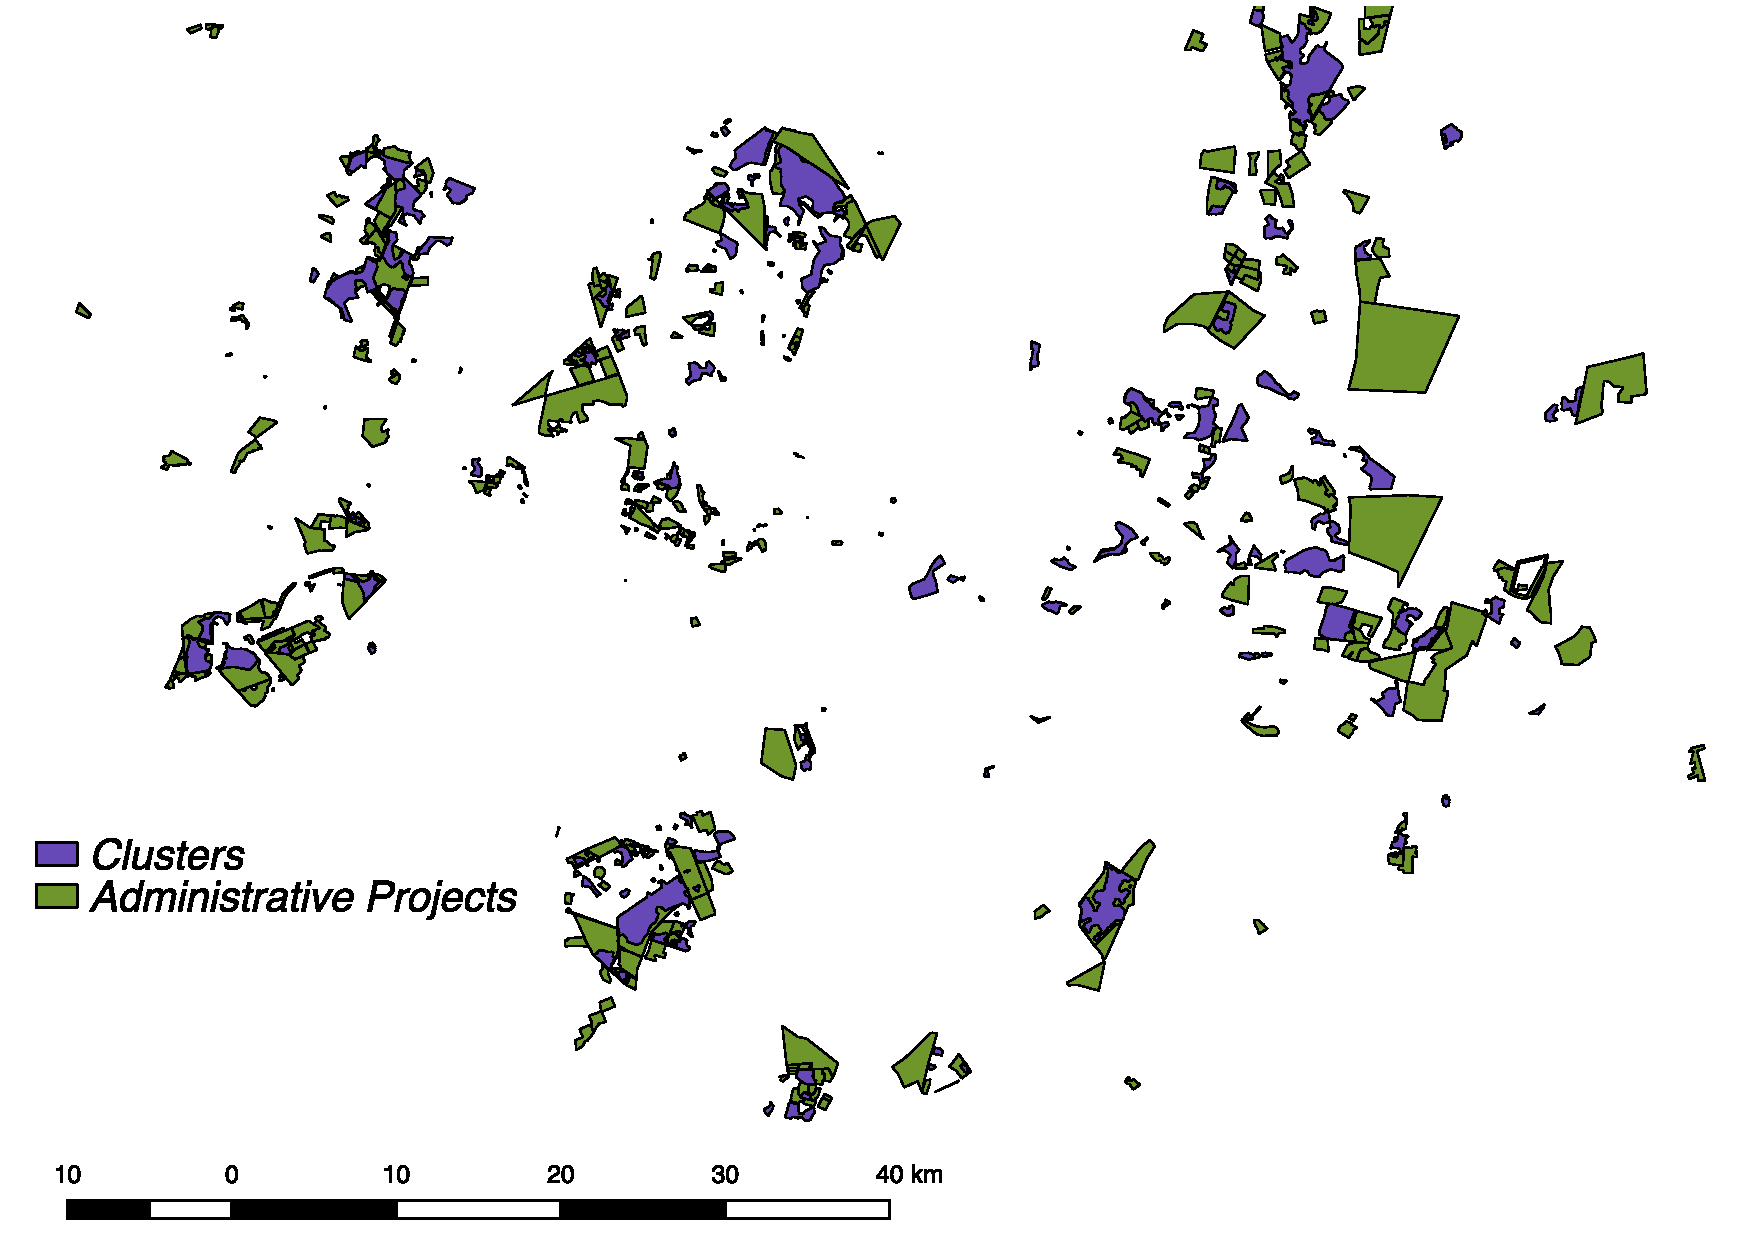
\includegraphics[scale=.5]{figures/gcro_convexhull_overlap.pdf} \\
% This figure includes the northern half of housing projects.
% \end{figure}

To contextualize our main analysis, we first provide descriptive evidence on the location, size, and surrounding housing stock of our 117 sampled housing projects. Table~\ref{table:projectdescriptives} reveals that constructed projects provide generous quantities of new housing, delivering on average more than 890 units per project. Constructed projects are also substantially larger in area than unconstructed projects. As mentioned in section \ref{section:data}, these discrepancies may be due to many unconstructed projects representing smaller planned extensions to previously implemented projects. \iffalse It may also reflect that larger land plots are first targeted by housing authorities to maximize delivery.\fi Though unconstructed projects are located in slightly more remote locations, both types of projects impose long commutes on residents, as measured by the average distance to central business districts. These distances are consistent with housing authorities targeting inexpensive, vacant land for these projects. Finally, prices for non-subsidized housing in the vicinity of project boundaries are slightly lower for unconstructed projects, perhaps driven in part by their more distant locations.


Next, we turn to household census data to assess how both types of projects differ in terms of dwelling characteristics prior to project construction. We identify census small areas as pertaining to a housing project when over 30\% of their land areas overlaps with a project boundary.\footnote{Our census geography selection method is depicted in more detail in appendix \ref{appendix:bufferdesign}.} This procedure results in 1,207 small areas containing a total of 257,997 households. Table \ref{table:projectdescriptivescensus} compares various indicators for these households on the basis of whether they live within the boundaries of a constructed (first column) or planned but unconstructed project (second column). As a reference, the third column provides averages for every variable using the entire sample of Gauteng households in 2001. 
 

\begin{table}[h!]
	\centering
	\caption{Dwelling Characteristics at Baseline from 2001 Census}\label{table:projectdescriptivescensus}
\vspace{-2mm}
\begin{tabular}{l*{1}{ccc}}
\toprule
& Constructed & Unconstructed & All Households \\
\midrule
Flush Toilet&0.55&0.45&0.81 \\
Piped Water in Home&0.13&0.19&0.46 \\
Electricity for Cooking&0.32&0.37&0.72 \\
Electricity for Heating&0.29&0.35&0.70 \\
Electricity for Lighting&0.56&0.45&0.81 \\
Number of Rooms&2.74&2.49&3.57 \\
Household Size&3.43&3.19&3.19 \\
N&        196,467&         61,530&      2,344,122 \\
 
\bottomrule
\end{tabular}
\end{table}

A clear takeaway from table \ref{table:projectdescriptivescensus} is that dwelling quality at baseline for both constructed and unconstructed project areas is far worse than the average Gauteng dwel\-ling. Given the quality of land plots that were targeted by this policy, we expect project areas to lag behind other areas, and reflect more precarious housing conditions. We find that access to sanitation, water and electricity are between 30 and 70\% lower in both types of project areas relative to the province as a whole. Comparing constructed to unconstructed projects, we find no systematic differences in dwelling quality. While constructed areas are more likely to have flush toilets, electricity for lighting, and a larger number of rooms, households in unconstructed areas report having better access to piped water and electricity for heating and cooking. Despite similarities between averages in constructed and unconstructed areas, we note that a simple t-test rejects the null hypothesis that means are equal for every tabulated variable.\footnote{Row 3 of table \ref{table:censusestimates} tests identical null hypotheses in a regression framework that allows for arbitrary correlations between observations within the same project, and cannot reject equality for all outcomes except household size.}


\begin{figure*}[t!]
        \centering
        \caption[ Housing Densities in Constructed and Unconstructed Projects Areas ]
        {\small Housing Densities in Constructed and Unconstructed projects } 
        %\vspace{2mm}
        \begin{subfigure}[b]{0.495\textwidth}
            \centering
            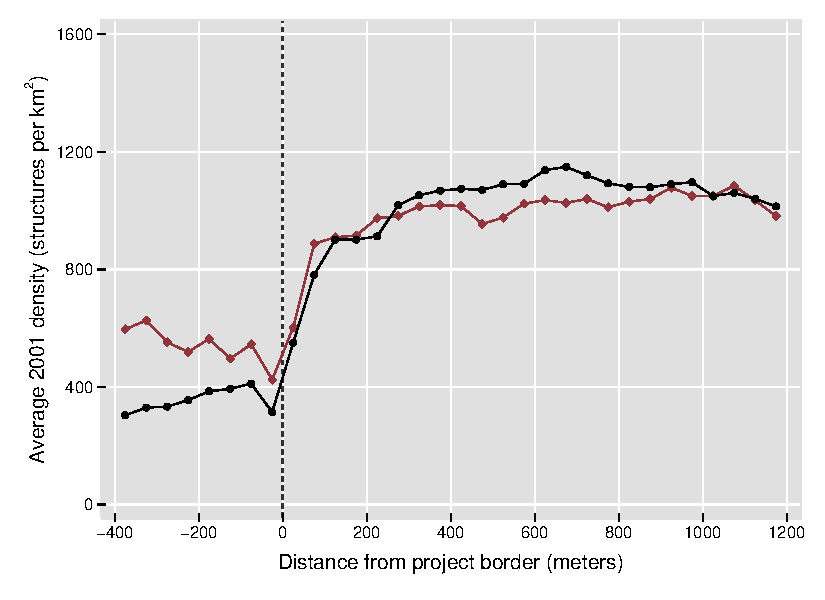
\includegraphics[width=\textwidth,trim={0.3cm .3cm 0.1cm 0cm}, clip=true]{figures/bblu_for_pre_means}
            \caption[Network2]%
            {{\small pre-period formal housing density}}    
            \label{fig:prefor}
        \end{subfigure}
        \hfill
        \begin{subfigure}[b]{0.495\textwidth}  
            \centering 
            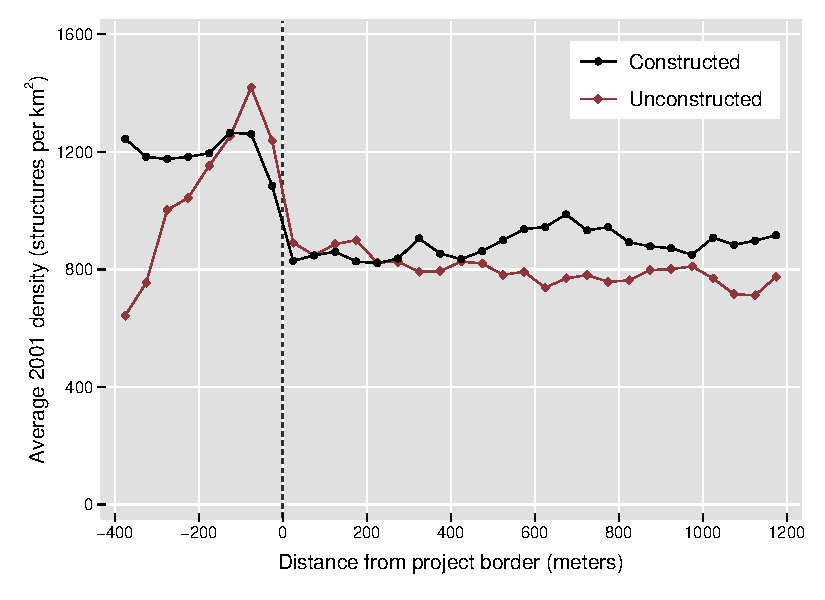
\includegraphics[width=\textwidth,trim={0.3cm .3cm 0.1cm 0cm}, clip=true]{figures/bblu_inf_pre_means}
            \caption[]%
            {{\small pre-period informal housing density}}    
            \label{fig:preinf}
        \end{subfigure}
        \vskip 1mm \vskip 0pt
        \begin{subfigure}[b]{0.495\textwidth}   
            \centering 
            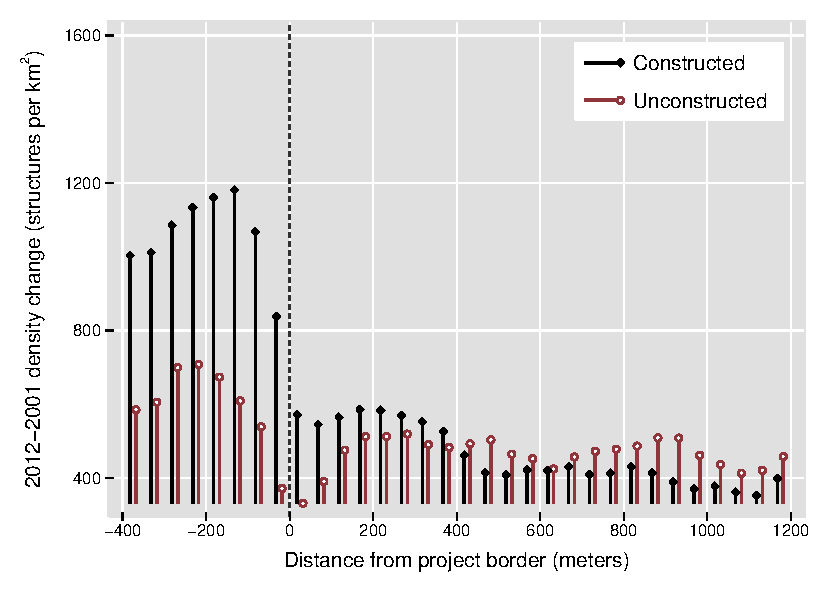
\includegraphics[width=\textwidth,trim={0.3cm .3cm 0.1cm 0cm}, clip=true]{figures/bblu_for_rawchanges}
            \caption[]%
            {{\small formal housing density change}}    
            \label{fig:forchange}
        \end{subfigure}
        \hfill
        \begin{subfigure}[b]{0.495\textwidth}   
            \centering 
            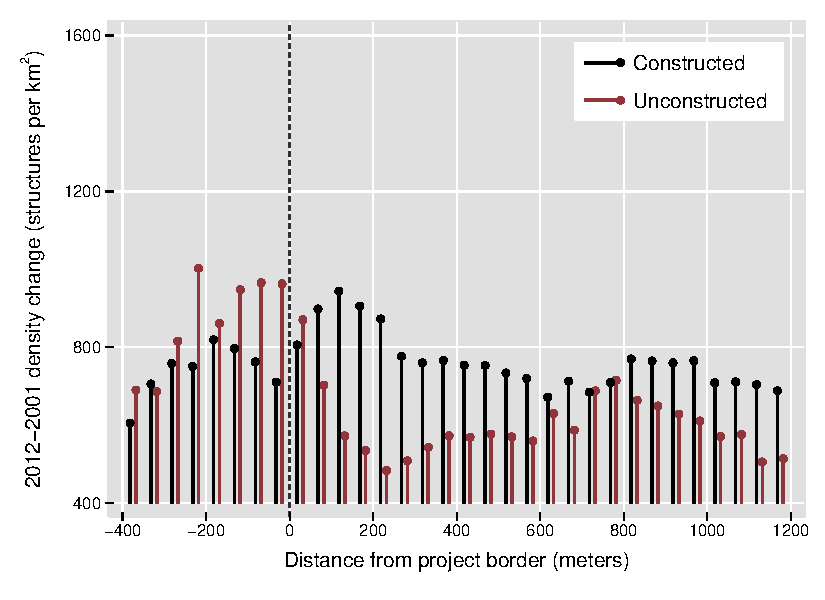
\includegraphics[width=\textwidth,trim={0.3cm .3cm 0.1cm 0cm}, clip=true]{figures/bblu_inf_rawchanges}
            \caption[]%
            {{\small informal housing density change}}    
            \label{fig:infchange}
        \end{subfigure}
        \label{fig:rawbblumeans}
        \vspace{-6mm}
    \end{figure*} 

Using the building-based land-use measures described in section \ref{section:data:bblu}, we then examine housing densities across constructed and unconstructed project areas.  To inspect how densities change with proximity to housing projects, we calculate euclidean distances from the centroid of each 50m$\times$50m grid-cell to the nearest project boundary. We assign negative distances to grid-cells lying inside these boundaries.  We then compute the average density at 50m intervals, reported in structures per square kilometer.  

Figures \ref{fig:prefor} and \ref{fig:preinf} respectively plot average densities of formal and informal houses in the pre-period. In Figure \ref{fig:prefor}, we find low densities of formal housing within both unconstructed and constructed project areas. This finding is consistent with governments locating projects on underdeveloped land.  Moving outwards, formal housing density jumps sharply at project boundaries and quickly stabilizes at a higher level across positive distances.  Figure \ref{fig:preinf} reports an inverse pattern for informal housing, with high levels of informal housing sharply declining just outside of project boundaries.\footnote{Greater negative distances exclude smaller projects in computing average density, which may account for some of the variation in building density within projects.  Appendix~\ref{appendix:projectcounts} illustrates this compositional change in more detail.}

We find relatively flat trends in housing density just outside of project boundaries across all categories (formal and informal housing for both constructed and unconstructed projects).  
%This cross-sectional evidence already suggests that living next to project areas at baseline (with high relative densities of informal dwellings) may not have strong effects on local development; if vacant land acts as a negative amenity, we would have expected to see much lower housing densities just nearby project boundaries.  From an empirical perspective, 
Similar levels of baseline densities near and far from boundaries provide suggestive evidence that these housing markets were following similar trajectories before the designation of projects.  This finding supports our identification strategy of attributing differential changes with respect to project proximity to the spillover effects of housing projects.  Similar logic applies for comparing constructed and unconstructed projects: their almost identical density patterns at baseline support the assumption that later deviations in housing markets between constructed and unconstructed areas are solely due to project completion.

Figures \ref{fig:forchange} and \ref{fig:infchange} extend this exercise by plotting average changes in housing densities between 2001 and 2012. The effect of the policy is clearly evidenced in figure \ref{fig:forchange}, where tall black bars at negative distances show increases in the density of formal housing of around 1,000 structures per $\text{km}^{2}$ within constructed project areas.  Compared to a baseline mean density of about 400 structures per $\text{km}^{2}$ in Figure \ref{fig:prefor}, this shift represents a nearly 250\% increase. In contrast, unconstructed areas (red bars) experience increases in formal housing density at much smaller rates.
%Importantly, density changes at negative distances for unconstructed areas resemble changes outside of project areas in magnitude, consistent with a broader secular expansion in housing.
At positive distances, both series are almost overlapping.  This result previews our empirical analysis by showing little evidence of spillover effects on neighboring formal housing markets.

In figure \ref{fig:infchange}, we observe large increases in informal density within project boundaries for both constructed and unconstructed project areas.  At some distances, unconstructed projects appear to overtake constructed areas in informal housing growth.  Outside of project boundaries, constructed areas experience larger increases in informal density than unconstructed areas. With the exception of 0-200m, these increases do not appear to be systematically different between the treated and control ares. 
%This absence of differential trends with distance previews a similar absence of spillover effects for informal housing densities explored further in the empirical analysis.
Relative to baseline levels in Figure \ref{fig:preinf}, informal housing increases are large, increasing by at least 50\% across all distances and nearly doubling in some cases.

Figure~\ref{fig:rawpricemeans} performs an analogous exercise with property transaction data from the deeds records.  These records are likely to be composed of formal houses because informal housing transactions are rarely recorded.  Since there are very few non-subsidized housing transactions within project footprints, we focus only on transactions at positive distances.  Using the date of each transaction, we group prices before and after the expected completion dates for both constructed and unconstructed projects. To make comparisons within a normalized timeline, we first residualize log purchase prices from year$\times$month and project fixed effects.

\begin{figure*}[b!]
        \centering
        \caption[ House Prices outside Constructed and Unconstructed Projects Areas ]
        {\small House Prices outside Constructed and Unconstructed projects } 
        %\vspace{2mm}
        \begin{subfigure}[b]{0.495\textwidth}
            \centering
            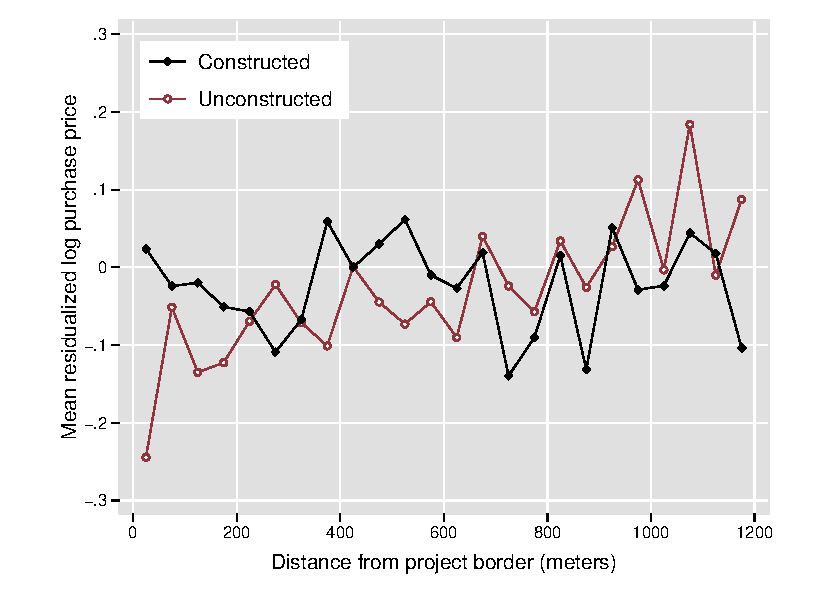
\includegraphics[width=\textwidth,trim={0.9cm .3cm 0.1cm 0cm}, clip=true]{figures/price_pre_means}
            \caption[Network2]%
            {{\small pre-period log-purchase prices }}    
            \label{fig:preprice}
        \end{subfigure}
        \hfill
        \begin{subfigure}[b]{0.495\textwidth}   
            \centering 
            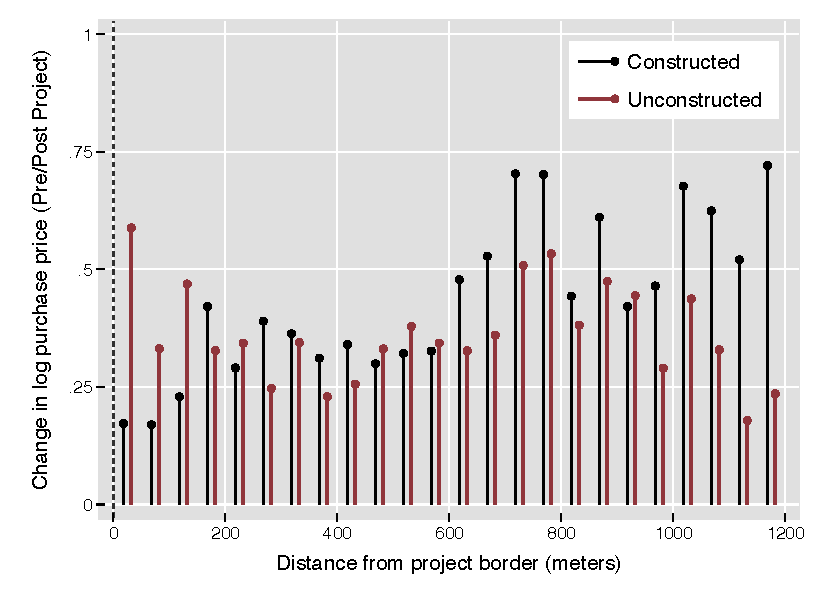
\includegraphics[width=\textwidth,trim={0.9cm .3cm 0.1cm 0cm}, clip=true]{figures/prices_rawchanges}
            \caption[]%
            {{\small change in log-purchase prices}}    
            \label{fig:changeprice}
        \end{subfigure}
        \label{fig:rawpricemeans}
        \vspace{-6mm}
\end{figure*} 


Figure~\ref{fig:preprice} plots average residualized log purchase prices before the expected completion date for both constructed and unconstructed areas. We document an increase in prices of about 0.2 log-points or roughly 20\% for unconstructed project areas. The picture is less clear for constructed projects, which show an increasing price gradient within the first 500m, but exhibit noisy patterns further away.  Overall, both series show large variations in house prices, but do not appear to diverge significantly at a any distance. The steady increase observed for unconstructed project areas is consistent with findings in table \ref{table:projectdescriptivescensus} that project areas (both constructed and unconstructed) fare worse in terms of indicators of dwelling quality.

Finally, figure~\ref{fig:changeprice} graphs average changes in log-purchase prices before and after the expected completion of projects. Both series are once more quite noisy. Under 400 meters, we observe some evidence that unconstructed areas experience a boom in nearby housing prices that was not mirrored by constructed areas.  Yet, this gap quickly closes, further suggesting that housing projects play a minimal role in driving nearby housing markets.


\section{Estimation Results}\label{section:results}

To draw statistical inference on the patterns depicted in section \ref{section:descriptives}, we proceed to estimate variants of equation (\ref{eq:main}) for each outcome of interest. 


\subsection{Infrastructure and Demographic Effects}\label{section:resultscensus}

\afterpage{%
  \clearpage% 
\begin{landscape}
{\footnotesize
\begin{table}[]
\small
\centering
\caption{Census Household-level Estimates}\label{table:censusestimates}
\vspace{-2mm}
\begin{tabular}{lDDDDDDDD}
\toprule
 & \small (1) & \small (2)  & \small (3) & \small (4) & \small (5)  & \small (6)  & \small (7) & (8)\\
 & \small Flush Toilet & \small Water Indoors  & \small Electricity Cooking & \small Electricity Heating & \small Electricity Lighting  & \small Number of Rooms  & \small Household Size & Population Density\\ \midrule 
project{\tim}post{\tim}constr&       0.123\textsuperscript{c}&       0.138\textsuperscript{a}&       0.284\textsuperscript{a}&       0.197\textsuperscript{a}&       0.101                   &      -0.132                   &      -0.233\textsuperscript{b}&      99.563                   \\
            &     (0.064)                   &     (0.051)                   &     (0.068)                   &     (0.065)                   &     (0.078)                   &     (0.185)                   &     (0.117)                   &  (1448.879)                   \\[0.5em]
project{\tim}post&       0.082\textsuperscript{c}&       0.099\textsuperscript{a}&       0.182\textsuperscript{a}&       0.157\textsuperscript{a}&       0.157\textsuperscript{b}&       0.480\textsuperscript{a}&      -0.039                   &    2320.431\textsuperscript{b}\\
            &     (0.048)                   &     (0.038)                   &     (0.060)                   &     (0.056)                   &     (0.066)                   &     (0.118)                   &     (0.055)                   &  (1111.722)                   \\[0.5em]
project{\tim}constr&       0.106                   &       0.001                   &      -0.042                   &      -0.038                   &       0.153                   &       0.255                   &       0.503\textsuperscript{a}&    -611.013                   \\
            &     (0.113)                   &     (0.086)                   &     (0.110)                   &     (0.094)                   &     (0.128)                   &     (0.258)                   &     (0.125)                   &  (1733.494)                   \\[0.5em]
project     &      -0.333\textsuperscript{a}&      -0.226\textsuperscript{a}&      -0.360\textsuperscript{a}&      -0.321\textsuperscript{a}&      -0.370\textsuperscript{a}&      -1.034\textsuperscript{a}&      -0.397\textsuperscript{a}&     416.265                   \\
            &     (0.078)                   &     (0.053)                   &     (0.070)                   &     (0.063)                   &     (0.081)                   &     (0.165)                   &     (0.080)                   &   (691.463)                   \\[0.5em]
spillover{\tim}post{\tim}constr&       0.034                   &       0.032                   &       0.036                   &      -0.041                   &      -0.024                   &       0.036                   &      -0.118\textsuperscript{b}&     444.064                   \\
            &     (0.034)                   &     (0.033)                   &     (0.033)                   &     (0.045)                   &     (0.030)                   &     (0.088)                   &     (0.047)                   &   (470.258)                   \\[0.5em]
spillover{\tim}post&       0.044\textsuperscript{c}&       0.135\textsuperscript{a}&       0.124\textsuperscript{a}&       0.102\textsuperscript{a}&       0.084\textsuperscript{a}&       0.229\textsuperscript{a}&      -0.151\textsuperscript{a}&     652.913\textsuperscript{b}\\
            &     (0.024)                   &     (0.025)                   &     (0.027)                   &     (0.023)                   &     (0.027)                   &     (0.053)                   &     (0.035)                   &   (325.594)                   \\[0.5em]
spillover{\tim}constr&      -0.020                   &      -0.038                   &      -0.051                   &      -0.025                   &       0.031                   &      -0.201\textsuperscript{c}&       0.153\textsuperscript{a}&     -23.442                   \\
            &     (0.061)                   &     (0.051)                   &     (0.050)                   &     (0.049)                   &     (0.064)                   &     (0.119)                   &     (0.049)                   &  (1353.816)                   \\ \midrule
{\it p}-val, h\textsubscript{0}: project=spill. &       0.157                   &       0.046                   &       0.000                   &       0.000                   &       0.120                   &       0.298                   &       0.270                   &       0.811                   \\
Mean Outcome 2001&        0.71                   &        0.30                   &        0.58                   &        0.55                   &        0.72                   &        3.16                   &        3.48                   &    7,313.26                   \\
Mean Outcome 2011&        0.81                   &        0.48                   &        0.81                   &        0.69                   &        0.83                   &        3.34                   &        3.11                   &    9,118.36                   \\
R$^2$       &       0.274                   &       0.166                   &       0.246                   &       0.181                   &       0.217                   &       0.141                   &       0.047                   &       0.398                   \\
\# projects &         117                   &         117                   &         117                   &         117                   &         117                   &         117                   &         117                   &                               \\
N project areas&     758,773                   &     758,773                   &     758,773                   &     758,773                   &     758,773                   &     727,242                   &     754,430                   &                               \\
N spillover areas&   1,208,333                   &   1,208,333                   &   1,208,333                   &   1,208,333                   &   1,208,333                   &   1,136,228                   &   1,197,515                   &                               \\
N           &   1,967,106                   &   1,967,106                   &   1,967,106                   &   1,967,106                   &   1,967,106                   &   1,863,470                   &   1,951,945                   &       9,612                   \\

\bottomrule
\multicolumn{9}{l}{\footnotesize All regressions include project Fixed-Effects. Standard errors clustered at the project level in parenthesis. \textsuperscript{c} p$<$0.10,\textsuperscript{b} p$<$0.05,\textsuperscript{a} p$<$0.01 }
\end{tabular}
\end{table}
}
\end{landscape}
}

To assess impacts on dwelling quality, we pool the 2001 and 2011 census cross-sections and test for differential 10-year changes between constructed and unconstructed project areas. Because these data have coarser spatial resolutions, we define two levels of exposure to the policy: $D=\{\text{\small\it project},\text{\small\it spillover}\}$. As in table \ref{table:projectdescriptivescensus}, {\it project} households live in census small areas with over 30\% area overlap with project boundaries. The remaining {\it spillover} households live in small areas with less than 30\% area overlap, but whose centroids still fall within 1.5 km of a project boundary. Appendix \ref{appendix:bufferdesign} illustrates an example of these two definitions for a given constructed project. Our estimating equation is:

\vspace{-4mm}

\begin{equation}\label{eq:censushh}
\quad y_{ipt} \, = \, \lambda_{p} \,+\, \sum\limits_{\substack{d\in \{project,\\ spillover\}}} I^d_{ip}\Big( \alpha^d \textsc{\small Post}_{pt}\times\textsc{\small Const}_{p} \, + \, \beta^d\textsc{\small Post}_{pt} \, + \, \gamma^d\textsc{\small Const}_{p} \,\Big) + \, \theta I^{project}_{ip} \, +  \, \varepsilon_{ipt} \quad 
\end{equation}

\noindent where 2001 households inside {\it spillover} small areas for unconstructed projects are the omitted category. We estimate equation (\ref{eq:censushh}) using the same binary outcomes tabulated in table \ref{table:projectdescriptivescensus}, with the addition of a population density variable computed at the small area level. We construct this additional outcome by computing the sum of household sizes  and dividing it by the square-kilometer area of the census small area. To allow for arbitrary correlations between observations within the same project area, we cluster standard errors at the project level. 

Table~\ref{table:censusestimates} provides estimates of $\alpha^d$, $\beta^d$, $\gamma^d$, and $\theta$ for each outcome. Rows 1 through 4 describe effects for households in our {\it project} exposure definition, while rows 5 through 7 describe effects for our {\it spillover} definition. Rows 3 and 7 respectively show that for both {\it project} and {\it spillover} exposures, the model cannot reject the null that treated and control areas are equal at baseline (in 2001). The difference-in-differences coefficients in the first row (project$\,\times\,$post$\,\times\,$const) document statistically significant improvements in access to services such as flush toilets, indoor water taps, and electricity.\footnote{With the exception of electricity for lighting, which falls short of the 10\% significance level. } With probability increases exceeding 10 percentage points, the economic magnitudes of these estimates are large, consistent with the policy successfully providing better housing. We note that households living within {\it project} exposure areas need not be direct recipients of government houses, since our definition is inclusive of indirect recipients such as backyard shack dwellers as well. 

We do not find corresponding effects for households in the vicinity of constructed projects. With the exception of number of rooms in column (6), row 5 of table \ref{table:censusestimates} detects no statistically significant effects for outcomes in {\it spillover} areas. Though 95\% confidence intervals admit sizeable positive effects, we can rule in most cases that this effect equals its {\it project} counterpart.\footnote{Row 8 of table~\ref{table:censusestimates} tests the hypothesis that the {\it project} and {\it spillover} DID effects are equal, and reports p-values from the associated F-test.} These results suggest that households adjacent to constructed projects are not incentivized to invest in higher housing quality. 


\subsection{Housing Density Effects}\label{section:bbluestimates}

We assess impacts on housing densities by estimating:

\vspace{-4mm}

\begin{equation} \label{eq:bblu}
\begin{aligned}
\quad y_{ipt} \, =& \, \lambda_{0} \,+\, \sum\limits_{d\in D\setminus\{1200m\}} I^d_{ip}\Big( \alpha^d \textsc{\small Post}_{pt}\times\textsc{\small Const}_{p} \, + \, \beta^d\textsc{\small Post}_{pt} \, + \, \gamma^d\textsc{\small Const}_{p} \, + \, \theta^{d} \Big) \\
& \, + \, \alpha^o \textsc{\small Post}_{pt}\times\textsc{\small Const}_{p} \, + \, \beta^o\textsc{\small Post}_{pt} \, + \, \gamma^o\textsc{\small Const}_{p} \, + \, \varepsilon_{ipt} \quad 
\end{aligned}
\end{equation}

\noindent Drawing from figure \ref{fig:rawbblumeans}, we define the set of distances $D$ as containing every 50m distance intervals from 400m inside project boundaries to 1200m outside project boundaries. Equation (\ref{eq:bblu}) departs from (\ref{eq:main}) in that coefficients $\alpha^d$ are expressed relative to the DID effect in the furthest distance bin, $\alpha^{1200m}$, which is normalized to zero. This rearrangement introduces  a third layer of differencing, comparing double-differences near versus far from project boundaries. A triple-differences strategy allows for differential trends between constructed and unconstructed projects, so long as these trends are identical $\forall d\in D$ in the absence of project construction. It further requires that any spillover effects fully dissipate within 1,200 meters from project boundaries, which figure~\ref{fig:rawbblumeans} supports.
%(2) differential shocks to local housing markets for constructed versus unconstructed projects are uncorrelated with distance within this radius, and (3) recipient households are not drawn from households living at 1,200 meters from the project area.

\begin{figure*}[t!]
    \centering
    \vspace{2mm}
    \begin{subfigure}[b]{0.49\textwidth}
        \centering
        \caption[]{\small Total Houses}  
        \vspace{-1mm}
        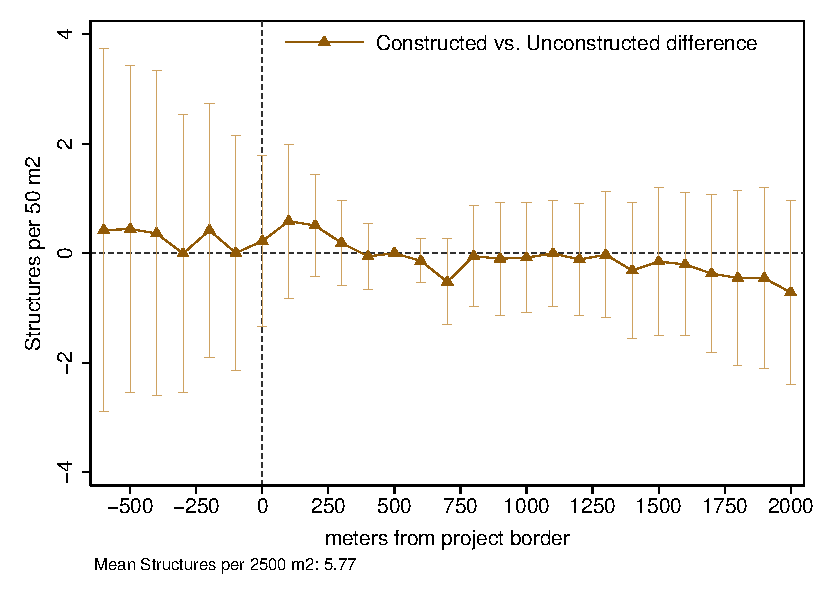
\includegraphics[width=\textwidth,trim={.5cm .3cm .3cm 0cm}, clip=true]{figures/distplotDDD_bblu_total_buildings_admin}
        \label{fig:DDDtotal}
    \end{subfigure}
    \hfill
    \begin{subfigure}[b]{0.49\textwidth}  
        \centering 
        \caption[]{\small Formal Houses}
        \vspace{-1mm}
        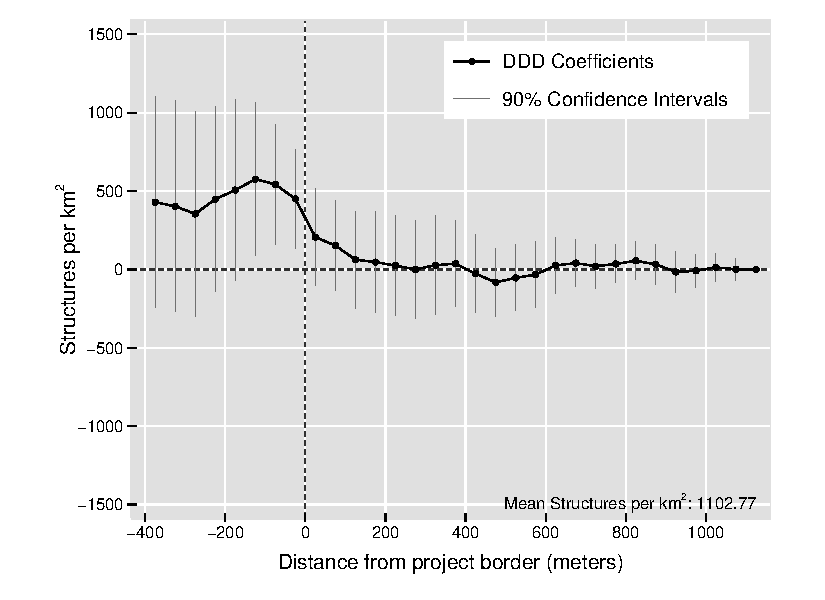
\includegraphics[width=\textwidth,trim={.5cm .3cm .3cm 0cm}, clip=true]{figures/distplotDDD_bblu_for_admin}     
        \label{fig:DDDformal}
    \end{subfigure}
    \vskip 1mm \vskip 0pt
    \begin{subfigure}[b]{0.49\textwidth}
        \centering
        \caption[]{\small Informal Houses}
        \vspace{-1mm}
        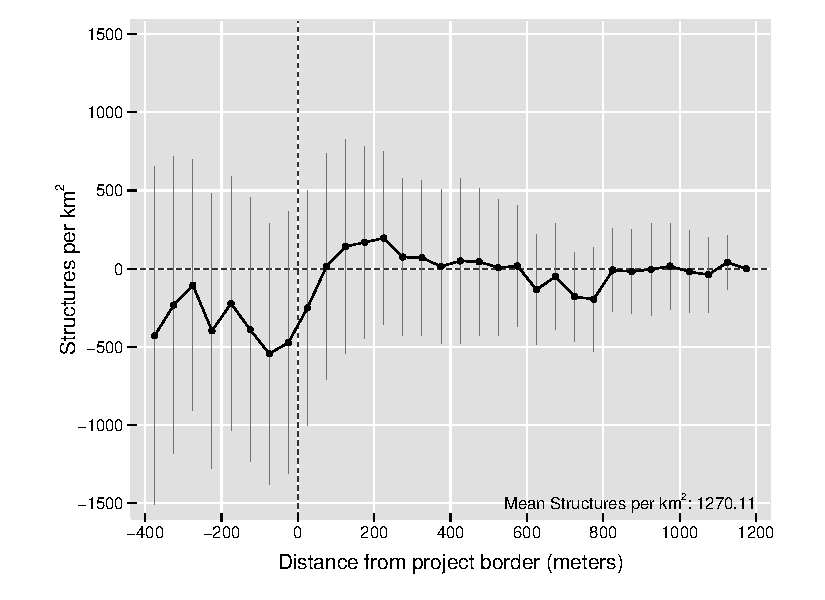
\includegraphics[width=\textwidth,trim={.5cm .3cm .3cm 0cm}, clip=true]{figures/distplotDDD_bblu_inf_admin.pdf}
        \label{fig:DDDinformal}
    \end{subfigure}
    \hfill
    \begin{subfigure}[b]{0.49\textwidth}  
        \centering
        \caption[]{\small Backyard Informal Houses}  
        \vspace{-1mm}
        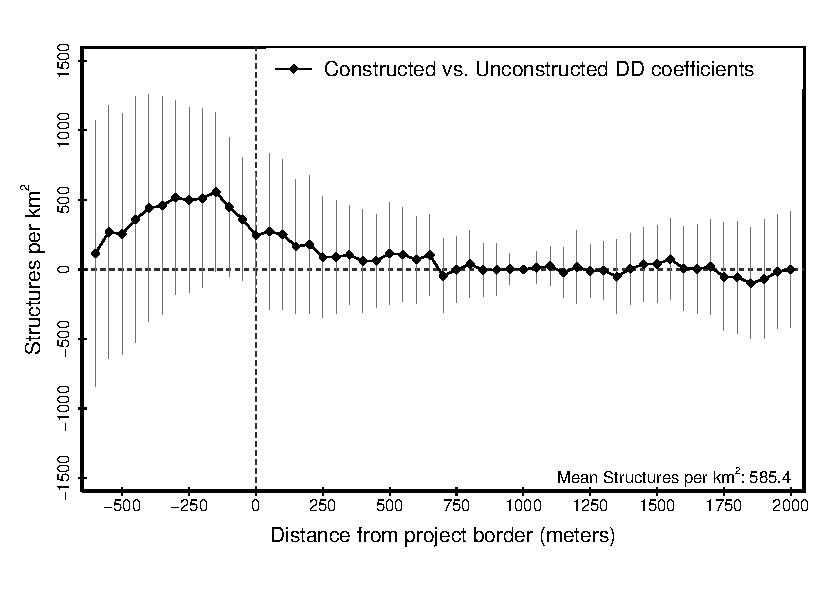
\includegraphics[width=\textwidth,trim={.5cm .3cm .3cm 0cm}, clip=true]{figures/distplotDDD_bblu_inf_backyard_admin}
        \label{fig:DDDbackyard}
    \end{subfigure}
    \vskip 1mm \vskip 0pt
    \begin{subfigure}[b]{.49\textwidth}  
        \centering
        \caption[]{\small Non-Backyard Informal Houses} 
        \vspace{-1mm}
        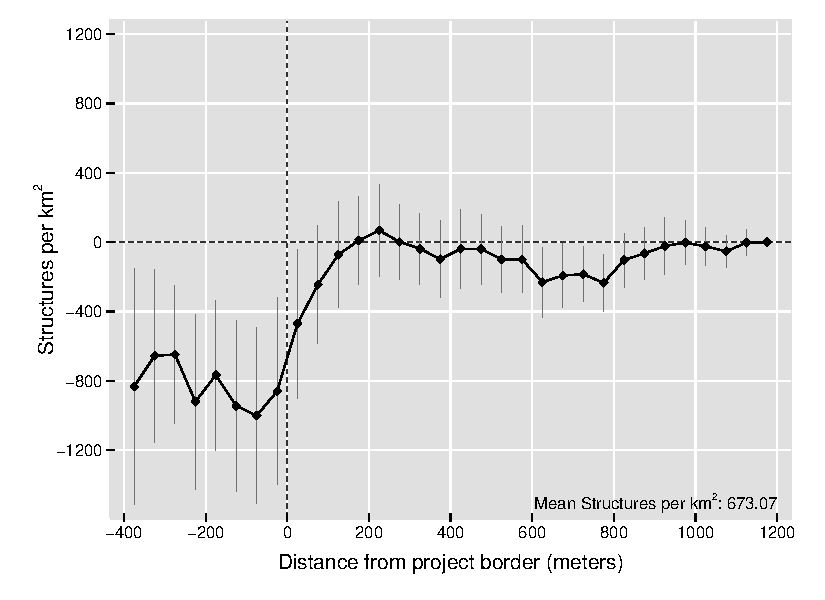
\includegraphics[width=\textwidth,trim={.5cm .3cm .3cm 0cm}, clip=true]{figures/distplotDDD_bblu_inf_non_backyard_admin}    
        \label{fig:DDDnonbackyard}
    \end{subfigure}
    \hfill \hspace{.02\textwidth}
    \begin{minipage}{0.47\textwidth}   
    \vspace{-6cm}
    \caption[]
    {\small DDD coefficients (equation \ref{eq:bblu}) for fives types of housing densities.} \label{fig:DDDbblu}
	\end{minipage}
\end{figure*} 

We estimate impacts on five housing density measures: 1) total houses, 2) formal houses, 3) informal houses, which are divided into 4) backyard shacks and 5) informal non-backyard houses.  Figure~\ref{fig:DDDbblu} plots the $\alpha^{d}$ coefficients across all outcomes for distance bins within projects (negative distances) and outside projects (positive distances). We accompany figure~\ref{fig:DDDbblu} with table~\ref{table:bbluDDD}, which provides point-estimates and standard errors for wider 400m distance bins relative to the omitted category [400m,1200m]. As in our previous estimation, we cluster standard at the project level for all regressions.


Figure~\ref{fig:DDDtotal} finds weak increases in total housing within and just outside ($\leq\,$200 meters) of projects before settling to zero at all greater distances.  Predicting increases of around 200 houses per kilometer near the project boundary, these coefficients are both statistically and economically insignificant given an average density of nearly 2,400 structures per kilometer.  

After measuring substantial numbers of houses per project in the descriptive evidence (Table~\ref{table:projectdescriptives}), it is surprising to find little evidence of housing spikes in these areas; however, the small effects on aggregate housing density mask larger shifts in the composition of housing.  Figure~\ref{fig:DDDformal} estimates over 30\% increases in formal housing density within project areas, which quickly dissipates just beyond their boundaries.  Coefficients within 200 meters inside the boundary are statistically different from those furthest away at the 10\% level.  Gains in formal housing density are almost entirely offset by losses in informal housing density as demonstrated by Figure~\ref{fig:DDDinformal}.  Informal housing density also seems to increase slightly just outside of project areas before stabilizing at zero growth further away.  Disaggregating informal housing further between backyard houses (Figure~\ref{fig:DDDbackyard}) and non-backyard houses (Figure~\ref{fig:DDDnonbackyard}) indicates that massive declines in non-backyard housing (of around 100\% of the average) are only partially offset by an almost doubling of the densities of backyard housing within projects.  Backyard housing growth extends slightly outside of the project boundary, accounting for the small increases in total housing observed in these regions (Figure~\ref{fig:DDDtotal}).


\begin{table}[h!]
\small
\centering
\caption{Triple Difference Estimates }\label{table:bbluDDD}
\vspace{-2mm}
\begin{tabular}{lCCCCC}
\toprule
& \small (1) & \small (2) & \small (3) & \small (4)& \small (5) \\
 & \small Total Housing & \small Formal Housing & \small Informal Housing & \small Backyard Housing & \small Non-Bkyrd Housing \\ \midrule 
-400m to 0m &      121.01   &      504.38** &     -383.37   &      419.94** &     -803.31***\\
            &    (296.06)   &    (206.69)   &    (292.55)   &    (181.72)   &    (265.47)   \\[0.5em]
0m to 400m  &      123.01   &       53.77   &       69.24   &       54.40   &       14.83   \\
            &    (148.32)   &    (104.60)   &    (148.03)   &    (130.97)   &    (114.79)   \\ \midrule
Mean dep. var.&    2,372.89   &    1,102.77   &    1,270.11   &      597.04   &      673.07   \\
\# Projects &         111   &         111   &         111   &         111   &         111   \\
R$^2$       &       0.098   &       0.116   &       0.055   &       0.101   &       0.044   \\
N           &     244,312   &     244,312   &     244,312   &     244,312   &     244,312   \\

\bottomrule
\multicolumn{6}{l}{\footnotesize Standard errors clustered at the project level in parenthesis. \textsuperscript{c} p$<$0.10,\textsuperscript{b} p$<$0.05,\textsuperscript{a} p$<$0.01 }
\end{tabular}
\end{table}

\subsection{Price Effects}\label{section:resultsprices}

To identify the spillover effects of public housing on local housing markets, our empirical strategy adopts the specification from Section~\ref{section:bbluestimates}, instead using transaction price as an outcome:
\begin{equation}
\label{equation:prices}
P_{ipt} \, = \sum\limits_{d} I^d_{ip}\Big( \alpha^d D_tC_p \, + \, \beta^dD_t \, + \theta^{d} \Big) \, + \, \lambda_p \, + \, \eta_t \, + \, X_i \, +  \, \varepsilon_{ipt}
\end{equation}

\begin{equation} \label{eq:bblu}
\begin{aligned}
\quad y_{ipt} \, =& \, \lambda_{0} \,+\, \sum\limits_{d\in D\setminus\{1200m\}} I^d_{ip}\Big( \alpha^d \textsc{\small Post}_{pt}\times\textsc{\small Const}_{p} \, + \, \beta^d\textsc{\small Post}_{pt} \, + \, \gamma^d\textsc{\small Const}_{p} \, + \, \theta^{d} \Big) \\
& \, + \, \alpha^o \textsc{\small Post}_{pt}\times\textsc{\small Const}_{p} \, + \, \beta^o\textsc{\small Post}_{pt} \, + \, \gamma^o\textsc{\small Const}_{p} \, + \, \varepsilon_{ipt} \quad 
\end{aligned}
\end{equation}

\noindent The outcome, $P_{itp}$, is measured in terms of the log-purchase price of property $i$ sold at time $t$ in the vicinity of project $p$.  Since we observe the exact transaction date, we set $D_{tp}$\,=1 if date $t$ is after the month of project implementation and zero otherwise.  As before, $C_{p}\,\,$=1 if project $p$ has been constructed and $I^d_{ip}$\,=1 if property $i$ is within distance bin $d$ of project $p$.  To account for smaller sample sizes than in the density estimation, we consider wider 200 meter distance bins from zero to 1200 meters.  Additionally, $\lambda_p$ includes a project fixed effect, controlling for any fixed, unobserved drivers of house prices that vary between projects.  Likewise, $\eta_{t}$ controls for year, year-month, and calendar month fixed effects depending on the specification to account for any factors such as shifts in aggregate housing demand that may be correlated with prices and the timing of housing projects.  To control for property characteristics, $X_i$ includes up to a cubic polynomial in lot size and a control for latitude-longitude cells in some specifications.  Each $\alpha^d$ captures the causal differences-in-differences effect for distance bin $d$ given that the parallel trends assumption also holds at each distance $d$.  

We normalize the last distance bin from 1,000 to 1,200 meters to be the reference category, leaving all other coefficients  $\alpha^{d \neq 1200}$  to be interpreted relative to this furthest category.  Under the additional assumption that areas in the reference category would have also followed parallel trends with respect to all other categories, this comparison again allows for a triple-differences interpretation.  

%%% Don't have to keep this paragraph, we sort of discuss it before, up to you
One concern is that our ability to distinguish between deeds pertaining to project houses and deeds associated with normal house transactions may be imperfect.  Without addressing this concern, we would mistakenly include project house transfers in our outcome measure of normal house transactions, which would substantially bias price effects.  To account for this possibility, we limit our sample to include only seller-names that appear less than 30 times in the data, excluding         28\unskip\% of transactions.  Alongside government housing projects, this approach also mainly excludes large housing developers.  Therefore, the results take a more narrow interpretation as the effect of housing projects on prices for small-scale property owners.  Removing these observations leaves a total sample of     87,253deeds transactions within 2,000 meters of a project boundary.  %%% not 100% sure these obs numbers are right...

\begin{figure}
\caption{Price Estimates over Distance from Project}\label{figure:distplot}
\centering
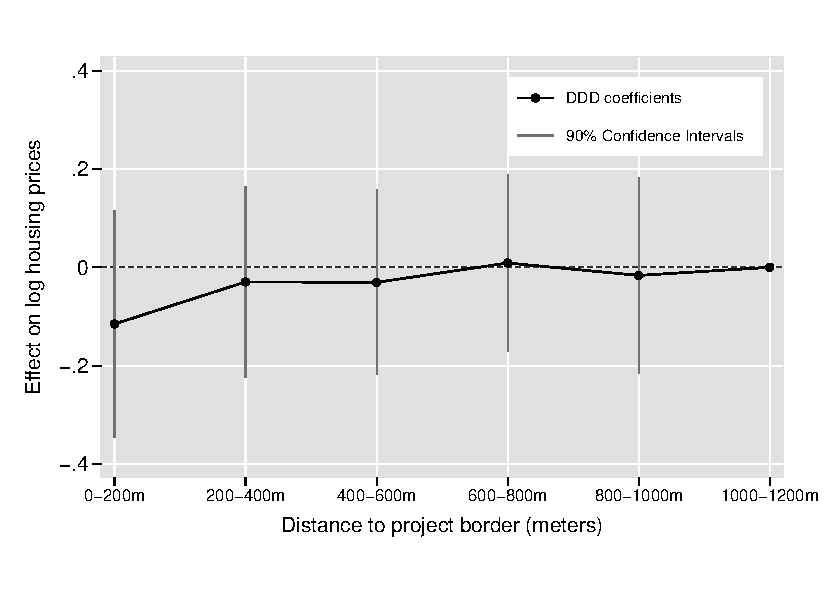
\includegraphics[width=0.9\textwidth,trim={0cm .7cm 0cm 0.7cm},clip=true]{figures/price_regs_DDDplot}
\vspace{-2mm}
\end{figure}

Figure~\ref{figure:distplot} plots the coefficients for differential changes in log-prices for constructed relative to unconstructed projects at a range of distances outside project boundaries.  This specification includes project as well as calendar month fixed effects and includes only transactions that occur within three years of project construction.  Examining the point estimates, we find evidence of a substantial drop in prices of around 0.1 log points or around 10\% within 200 meters of the project boundary.  Beyond 200 meters, this negative price effect disappears with all point estimates closely tracking zero.  With only 117 projects, clustering standard errors at the project level leaves wide confidence intervals at all distances, meaning that we are unable to reject equivalence between any coefficient and the price effect for the reference category at the 10\% confidence level.

\begin{figure}
\caption{Time-to-Event Price Estimates}\label{figure:timeplot}
\centering
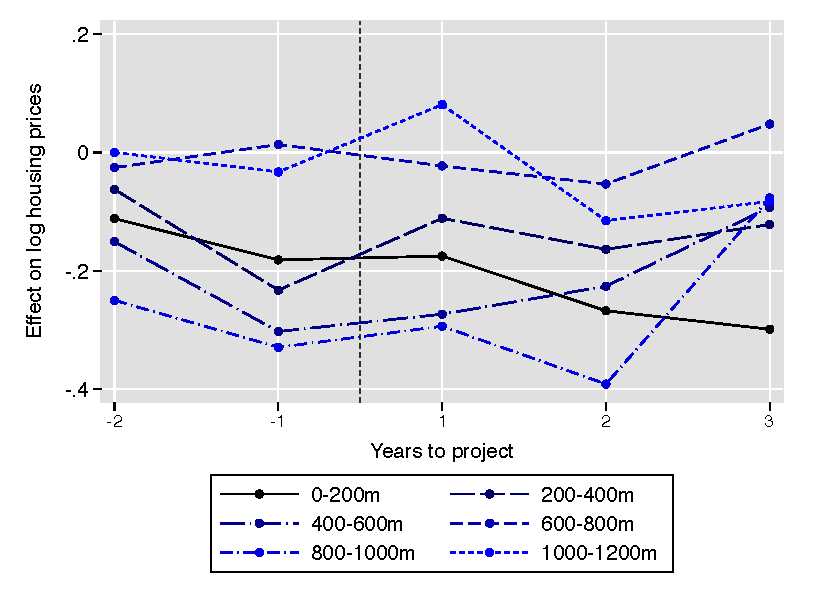
\includegraphics[width=0.9\textwidth,trim={0cm .1cm 0cm 0.1cm},clip=true]{figures/DDDplot_pertime_alt}
\vspace{-2mm}
\end{figure}

To examine how these effects evolve over time, we interact an indicator for successful construction with year dummies relative to the date of construction.  We also estimate these trends separately for six different distance bins relative to the project boundary.  Figure~\ref{figure:timeplot} plots these coefficients, excluding the confidence intervals.  Further splitting the sample for this exercise widens the confidence intervals so that all 90\% intervals contain zero.  We set the reference category to be two-years prior to project construction for the furthest distance bin.  

Examining the two years prior to construction, we see some evidence of anticipation with prices declining most steeply for distances within 600 meters of project construction.  After project construction, prices gradually recover to pre-project levels except for the closest distance bin (less than 200 meters) which continues to decline.  Time trends for distances beyond 600 meters appear relatively uncorrelated with the time of project completion, suggesting that these areas may be unaffected by project construction.

Table~\ref{table:priceDDD} provides point estimates for distance bins up to 600 meters across a variety of controls and using a broader reference category including all distances from 600 meters to 1,200 meters.  The first row confirms a price drop of around 10\% that is relatively stable as we include additional controls for project, time, and location.  We find much smaller but similarly negative price effects between 200 and 600 meters.  Wide standard errors ensure that no coefficients are statistically different from zero.

\begin{table}[h!]
\small
\centering
\caption{Triple Difference Estimates on Log-Prices}\label{table:priceDDD}
\vspace{-2mm}
\begin{tabular}{lCCCC}
\toprule
 & \small (1) & \small (2) & \small (3) & \small (4) \\ \midrule 
0 to 200m   &      -0.104&      -0.103&      -0.160&      -0.155\\
            &     (0.127)&     (0.093)&     (0.093)&     (0.118)\\[0.5em]
200m to 400m&      -0.061&      -0.058&      -0.111&      -0.104\\
            &     (0.099)&     (0.074)&     (0.084)&     (0.097)\\[0.5em]
400m to 600m&       0.057&       0.011&      -0.038&      -0.061\\
            &     (0.086)&     (0.077)&     (0.074)&     (0.073)\\ \midrule
Cubic in lot size&  \checkmark&  \checkmark&  \checkmark&  \checkmark\\
Project \textsc{FE}&           .&  \checkmark&           .&           .\\
Year{\tim}Project \textsc{FE}&           .&           .&  \checkmark&           .\\
Year{\tim}Lat-Lon cell \textsc{FE}&           .&           .&           .&  \checkmark\\
Year-Month \textsc{FE}&  \checkmark&  \checkmark&           .&           .\\
Month \textsc{FE}&           .&           .&  \checkmark&  \checkmark\\
R$^2$       &       0.174&       0.347&       0.381&       0.264\\
N           &     120,866&     120,866&     120,866&     120,866\\

\bottomrule
\multicolumn{5}{l}{\footnotesize Standard errors clustered at the project level in parenthesis. \textsuperscript{c} p$<$0.10,\textsuperscript{b} p$<$0.05,\textsuperscript{a} p$<$0.01 }
\end{tabular}
\end{table} 


\subsection{Composition}

To test whether housing projects induce sorting between project, spillover, and outside areas, we also examine how average demographics change as a result of these projects across these areas.  Appendix Table~\ref{appendix:censusperson} provides the differences-in-differences estimates for years of age, an indicator for place of birth outside of Gauteng province, an indicator for unemployment, years of education, and monthly income in Rands.  We detect no statistically or economically significant differential changes in average age and being born outside of Gauteng for both spillover and project areas.  However, we find that unemployment rates improve by 3.9 and 5.4 percentage points for project and spillover areas respectively.  Similarly, average years of education and monthly income both increase at similar magnitudes for both areas.  The unemployment and education interaction coefficients are statistically significant.  Taken together, these findings provide some evidence that more educated, higher income households are moving to constructed areas relative to unconstructed areas.  Yet, we cannot reject that these sorting patterns are different between spillover and project areas across any measures.%\footnote{The p-value reported in Appendix Table~\ref{table:censusperson} tests the equivalence of the ``Project $\times$ Post $\times$ Const.'' and ``Spillover $\times$ Post $\times$ Const.'' coefficients.}

\section{Conclusion}\label{section:discussion}

\begin{comment}

Our results present a puzzle: large improvements in housing quality and infrastructure access within projects do not appear to generate new investments in formal housing development, influxes of high-income residents, or increases in housing prices nearby these projects.  Additionally, we find no evidence that low-income households differentially sort into project areas or that projects increase the total supply of housing --- both mechanisms which may counteract any positive amenity effects.  We offer two partial explanations to account for this puzzle.

In making housing decisions, people in South Africa may simply have weak preferences for neighborhood quality.  Given very high rates of unemployment especially in rural areas, many South Africans migrate to cities solely for employment, sending large shares of their income home to their families.  In the census data, we observe that over 43\% of our sample reports being born outside the province of Gauteng.  Young adults regularly engage in circular migration, returning periodically to rural villages to spend their leisure time.  Rather than investing in the local community and developing a strong social network, people may view their housing decision in terms of short-term access to employment.  Therefore, people may place little value on nearby neighborhood quality or other amenities, instead prioritizing low rents and short commutes. 

Another explanation is that households value neighborhood quality, but higher densities of informal backyard shacks offset any improvements in formal housing quality and infrastructure.  \cite{Brueckner2018backyarding} document how households in backyard shacks often share water, electricity, and sanitation services with their landlords.  Congestion in using shared services may lead households to consume less of these services and exacerbate externalities associated with these low levels of usage.  \cite{Brueckner2018backyarding} also emphasize that backyard shacks often house young-adult, migrant workers who may be less inclined to make long-term social or economic investments in their communities.  

These results contrast with similar findings in both developed and developing country settings. - what papers to discuss?


Our interpretation is relatively neutral from a policy perspective: housing projects can produce enough positive amenities to mediate any housing supply effects.  Additionally, these projects effectively replace informal settlements with high quality formal houses, achieving a signature goal of South Africa's policy.  At the same time, there is little evidence supporting housing policy as an important engine for local economic growth and development.  These results may at least mediate any concerns policymakers may have for adversely affecting communities with housing projects, despite sometimes loud complaints from nearby community members.


It is important to emphasize that our analysis does not currently speak to the overall welfare implications of these policies.  Since project houses cannot be sold, we have difficulty measuring the extent to which households value these houses.  


Similarly, we do not measure the general equilibrium effects of housing policy outside of project neighborhoods; public housing may lead to an overall net reduction in slums in the city, which may generate total welfare gains through fewer congestion externalities or other mechanisms.  

In light of South Africa's emphasis on using housing policy to stimulate neighborhood development, we hope that this paper will be useful for policymakers in considering the range of informal housing market responses as they design new housing policies.

% We find that South African housing projects greatly improve the housing conditions within their footprints.  Housing projects successfully deliver large numbers of new formal structures (Figure~\ref{figure:dddformal}) and much better access to bulk services (Table~\ref{table:censusestimates}).  At the same time, formal project housing appears to crowd-out growth in informal settlements so that the total density of housing remains the same as in unconstructed project areas (Figure~\ref{figure:dddtotal}).  Moreover, results in Table~\ref{table:censusestimates} indicate that the average quality of new project houses are at least as good as neighboring houses at baseline.  Therefore consistent with the model of amenity effects in \cite{diamond2016wants}, we would expect to find that these programs increase nearby home prices; however, results in Table~\ref{table:priceest} report if anything the opposite trend.  Similarly, we do not observe large new developments in either informal or formal housing just nearby these projects.

% The lack of significant spillover effects in price as well as in quantity is consistent with countervailing amenity and housing supply effects.  While an influx of new houses threatens to decrease prices and housing supply nearby, positive amenities provided by housing projects may also attract greater housing investment, increasing prices.  While both amenity and supply effects predict increases in local population, there may be spatial or geographic constraints on population growth given that these settlements in South Africa are almost exclusively single-story and informal settlements often fill any remaining surface area.


%\section{Conclusion}\label{section:conclusion}
%This paper serves as a cautionary tale for low-density public housing in developing countries.  While these projects may be designed to improve local housing markets and reduce local slum growth, they may instead support local slum growth through a mix of available land and improved infrastructure.  It is important to emphasize that our analysis does not currently speak to the overall welfare implications of these policies.  For example, public housing may lead to an overall net reduction in slums in the city, which may generate total welfare gains through fewer congestion externalities or other mechanisms.  According to our model, the optimal housing policy depends crucially on the shape of these congestion externalities.  We look forward to using variation in the South African housing program to estimate these externalities in future work.  


% (1) construction costs, (2) value to recipients, (3) value to non-recipients within project footprints, and (4) spillover effects on neighboring areas.  


\end{comment}




\nocite{*}
\singlespacing
\setlength{\bibsep}{7pt}
\bibliographystyle{abbrvnat}
\bibliography{ref}



\pagebreak
% APPENDIX 
\appendix
\doublespacing

\section{Appendix}

\titleformat*{\subsection}{\centering\normalsize\bfseries}

\subsection{String Matching for Project Names and Delivery Dates }
\label{appendix:stringmatch}

\begin{center}
[...]
\end{center}



\begin{comment}

We then use a fuzzy-string matching algorithm with bigrams to link project names from the budget reports to the administrative maps.  We keep all matches with over 60\% similarity, with 44 projects matching exactly.  Appendix~\ref{table:stringmatch} compares unmatched and matched projects finding that matched projects have much higher densities of informal housing and project housing density, but similar densities of formal housing and project dates.  One reason may be that the budget reports only include larger, more expansive projects. We find that the project start date (from the budget reports) is three years before the project completion date (from the deeds data) on average.  In other words, beneficiaries receive title to their new houses about three years after the housing program is announced in the budget.  Using this lag, we assign an expected completion date for unconstructed projects that is three years after the announced start-date in the budget reports.  Since the budget data does not include month of planning, we assign a random month for unconstructed projects, which ensures that this date is uncorrelated with seasonality but also introduces measurement error in the timing of unconstructed projects.  This error is only likely to affect the housing transaction estimates, which are the only estimates performed at the monthly level.  

\begin{table}
	\centering
	\caption{Assessing Name Matching between \\Budget and Spatial Administrative Data}\label{table:stringmatch}
\begin{tabu}{lcc}
 & Matched  & Unmatched  \\
\midrule
 Formal Density: 2001  & 230.5  & 171.5  \\ 
 Formal Density: 2011  & 814.1  & 444.0  \\ 
 &  &  \\ 
 Informal Density: 2001  & 1,055.6  & 1,401.0  \\ 
 Informal Density: 2011  & 1,613.2  & 2,147.0  \\ 
 &  &  \\ 
 Project House Density  & 125.0  & 66.0  \\ 
 Project Mode Year  & 2005  & 2005  \\ 
 &  &  \\ 
 Hectares  & 97.3  & 119.6  \\ 
 &  &  \\ 
\midrule
 Observations  & 322  & 320  \\ 
\bottomrule
\end{tabu}
 \\
Density is measured in structures per $\text{km}^{2}$.
\end{table}
\end{comment}

\subsection{Buffer Design for Census Small Areas}
\label{appendix:bufferdesign}

\vspace{-3mm}

\begin{figure}[h!]
%\caption{Buffer Design for Census Small Areas}\label{figure:bufferdesigncensus}
\centering
\tcbox[colback=white,boxrule=.35mm,boxsep=0mm]{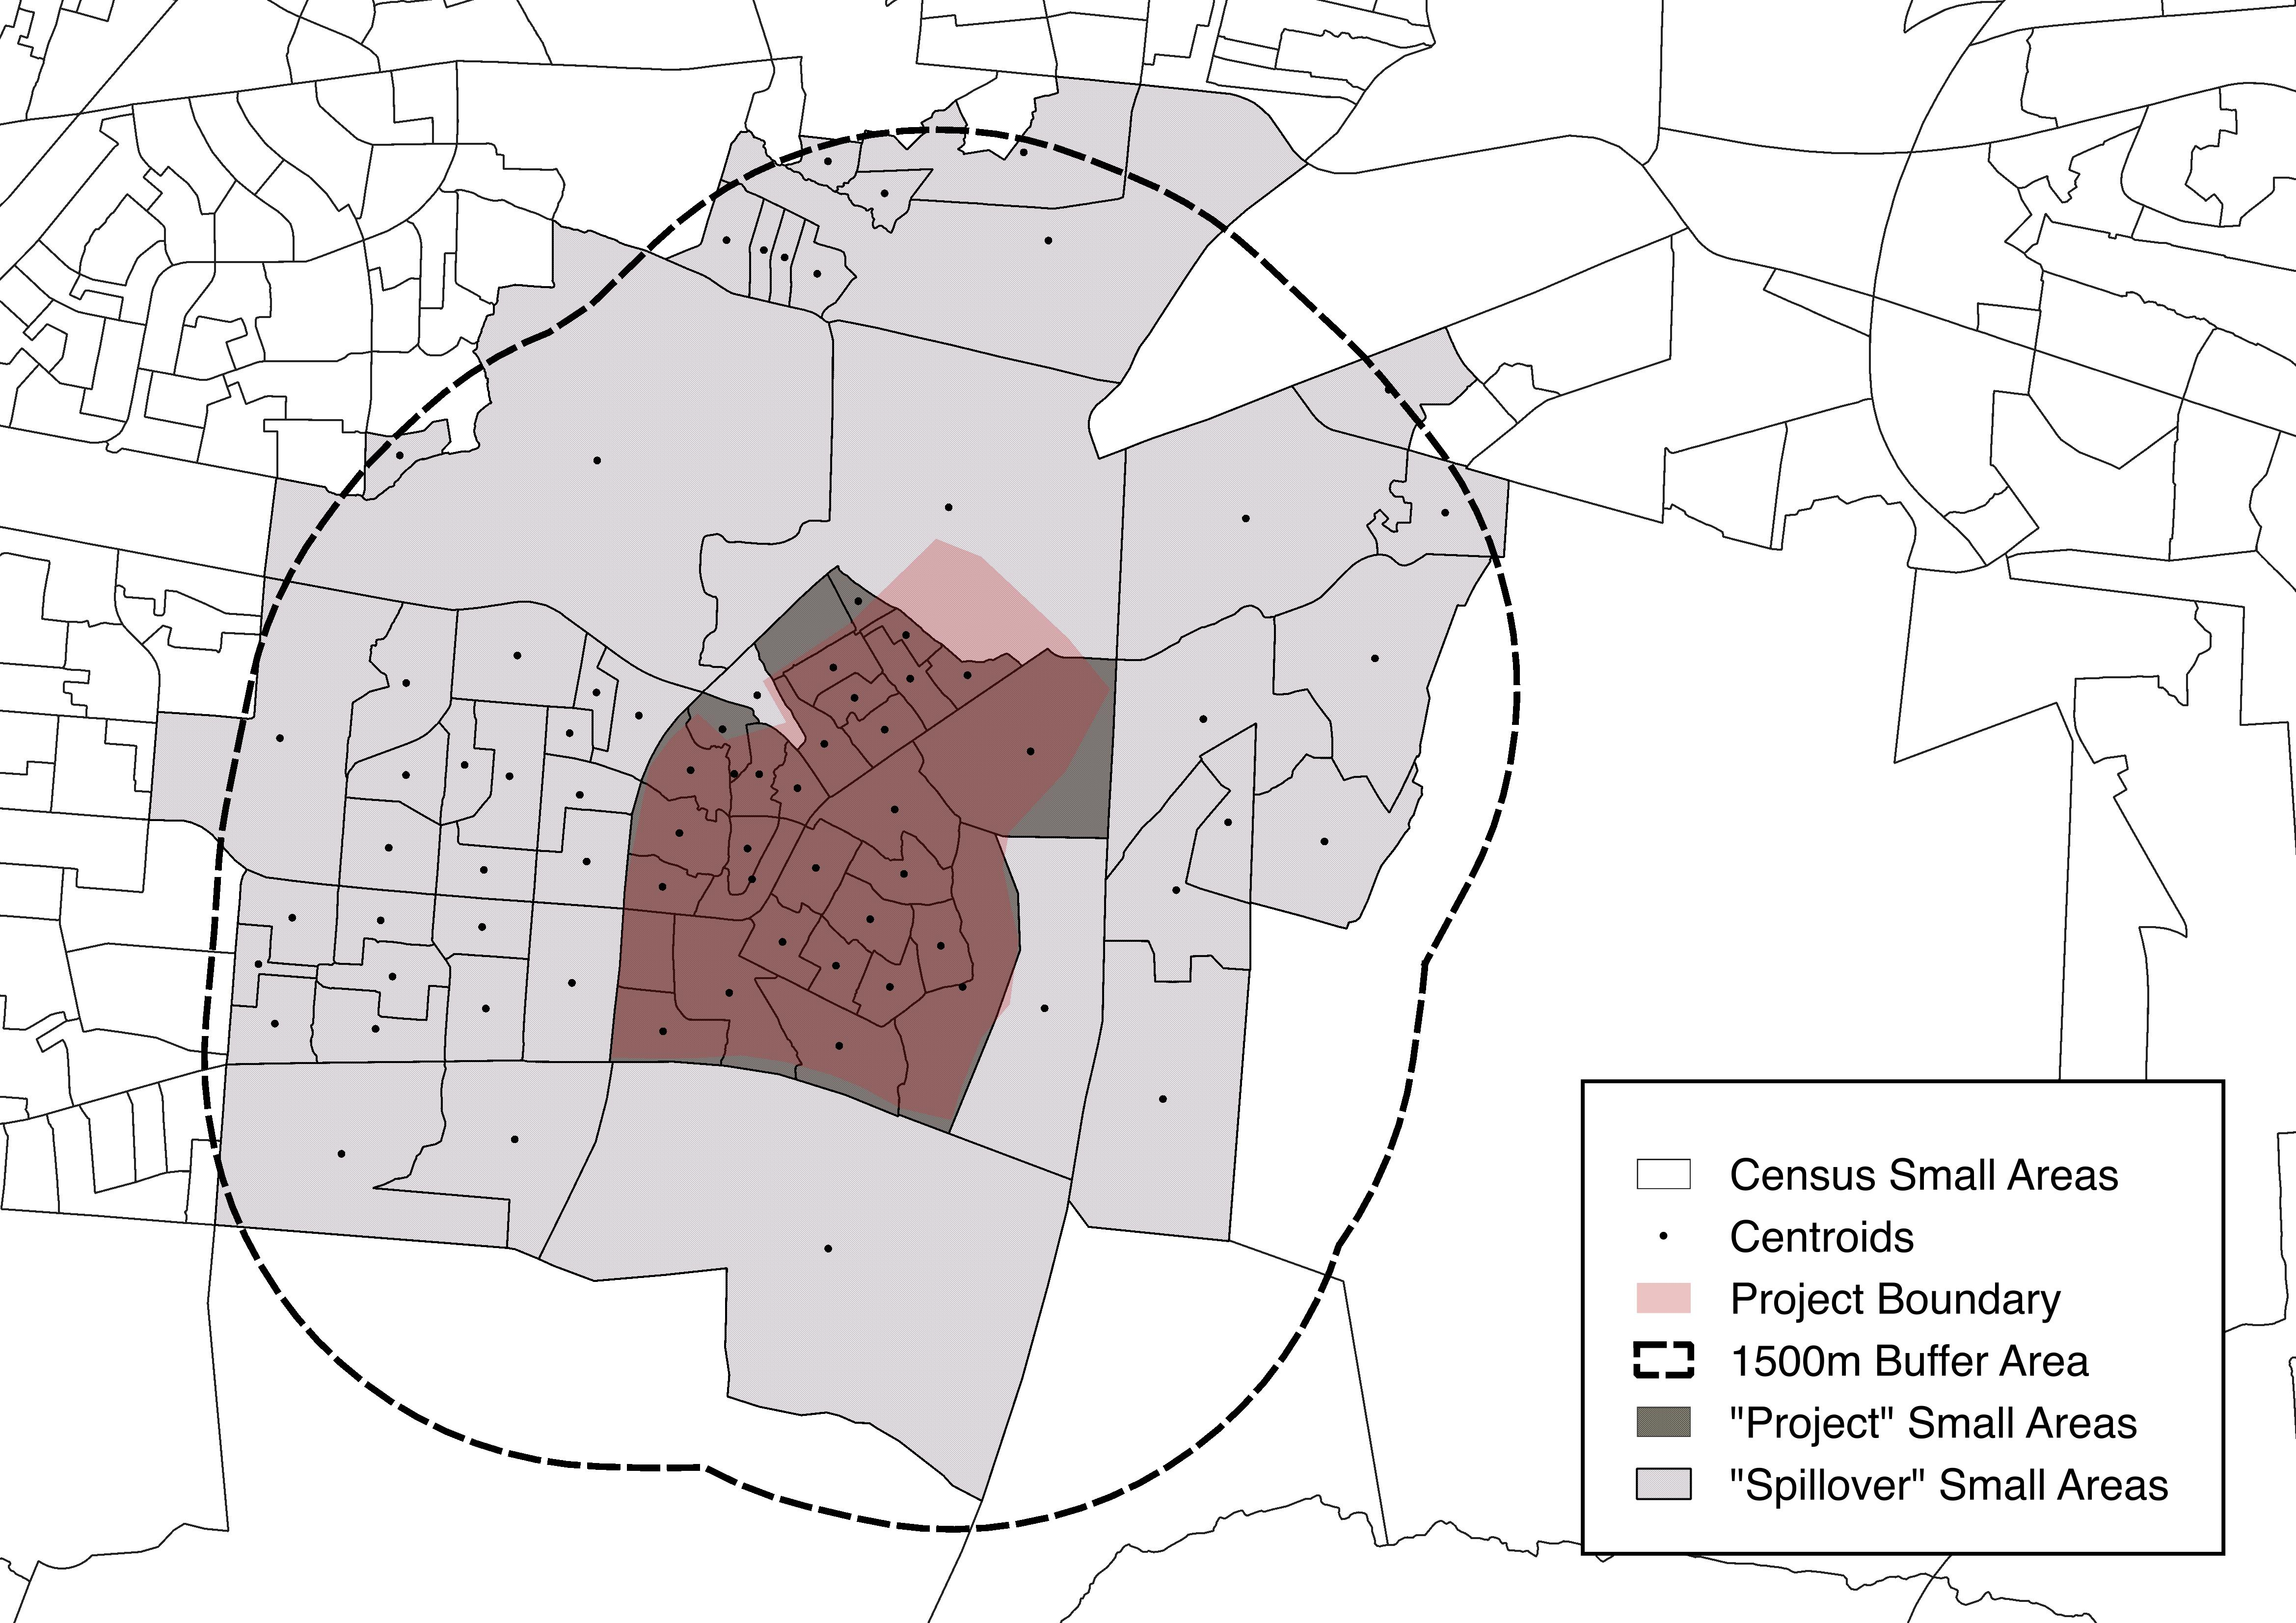
\includegraphics[scale=.47,trim={.75cm .4cm .75cm .4cm}]{figures/census_design.jpg}}
\vspace{2mm}
\caption*{\footnotesize {\bf Note:} We consider every census small areas whose centroid fall within 1500m of a project boundary. We denote small areas with over 30\% area overlap with project boundaries as "project" small areas, and use household responses within these geographies to capture dwelling characteristics inside project boundaries. All remaining small areas are denoted as "spillover" geographies, and are used to capture dwelling characteristics nearby.}
\end{figure}

\pagebreak

\subsection{Census Composition Estimates }
\label{appendix:censusperson}
\vspace{-5mm}
\begin{table}[h!]
\small
\centering
%\caption{Census Composition Estimates }
\vspace{-2mm}
\begin{tabular}{lDDDDD}
\toprule
& \small (1) & \small (2) & \small (3) & \small (4)& \small (5)\\
& \small Age & \small P.O.B. not Gauteng & \small Unemployed & \small Years of Education & \small Monthly Income \\ \midrule 
project{\tim}post{\tim}constr&       0.040                   &      -0.062                   &      -0.039\textsuperscript{c}&       0.053\textsuperscript{a}&     516.240                   \\
            &     (0.275)                   &     (0.059)                   &     (0.021)                   &     (0.013)                   &   (347.424)                   \\[0.5em]
project{\tim}post&       0.941\textsuperscript{a}&       0.004                   &      -0.106\textsuperscript{a}&       0.087\textsuperscript{a}&     143.066                   \\
            &     (0.250)                   &     (0.018)                   &     (0.012)                   &     (0.011)                   &   (260.514)                   \\[0.5em]
project{\tim}constr&      -0.653                   &       0.013                   &       0.024                   &      -0.045                   &      48.622                   \\
            &     (0.544)                   &     (0.053)                   &     (0.026)                   &     (0.034)                   &   (815.530)                   \\[0.5em]
project     &      -1.710\textsuperscript{a}&       0.133\textsuperscript{a}&       0.087\textsuperscript{a}&      -0.122\textsuperscript{a}&   -1413.068\textsuperscript{a}\\
            &     (0.293)                   &     (0.034)                   &     (0.018)                   &     (0.022)                   &   (433.012)                   \\[0.5em]
spillover{\tim}post{\tim}constr&       0.213                   &      -0.023                   &      -0.054\textsuperscript{a}&       0.031\textsuperscript{b}&     411.907                   \\
            &     (0.203)                   &     (0.030)                   &     (0.017)                   &     (0.014)                   &   (402.765)                   \\[0.5em]
spillover{\tim}post&       1.136\textsuperscript{a}&       0.021\textsuperscript{c}&      -0.086\textsuperscript{a}&       0.097\textsuperscript{a}&    1540.012\textsuperscript{a}\\
            &     (0.161)                   &     (0.011)                   &     (0.012)                   &     (0.011)                   &   (337.188)                   \\[0.5em]
spillover{\tim}constr&      -0.756\textsuperscript{b}&       0.011                   &       0.073\textsuperscript{a}&      -0.065\textsuperscript{a}&   -1012.065\textsuperscript{c}\\
            &     (0.293)                   &     (0.025)                   &     (0.016)                   &     (0.016)                   &   (511.127)                   \\ \midrule
{\it p}-val, h\textsubscript{0}: project=spill. &       0.574                   &       0.306                   &       0.466                   &       0.209                   &       0.821                   \\
Mean Outcome 2001&       26.55                   &        0.42                   &        0.50                   &        0.30                   &    2,333.46                   \\
Mean Outcome 2011&       27.62                   &        0.45                   &        0.34                   &        0.43                   &    3,848.70                   \\
R$^2$       &       0.009                   &       0.118                   &       0.041                   &       0.052                   &       0.030                   \\
\# projects &         117                   &         117                   &         117                   &         117                   &         117                   \\
N project areas&   1,786,402                   &   1,761,721                   &     851,435                   &   1,190,237                   &     702,249                   \\
N spillover areas&   3,062,022                   &   3,027,717                   &   1,449,407                   &   2,096,288                   &   1,205,674                   \\
N           &   4,848,424                   &   4,789,438                   &   2,300,842                   &   3,286,525                   &   1,907,923                   \\

\bottomrule
\multicolumn{6}{l}{\footnotesize Standard errors clustered at the project level in parenthesis. \textsuperscript{c} p$<$0.10, \textsuperscript{b} p$<$0.05, \textsuperscript{a} p$<$0.01  }\\
\multicolumn{6}{l}{\footnotesize P.O.B. means ``place of birth.''  Monthly income is in Rands.}
\end{tabular}
\end{table}


\pagebreak
\subsection{Project Counts}
\label{appendix:projectcounts}
\vspace{-5mm}
\begin{figure}[h!]
\centering
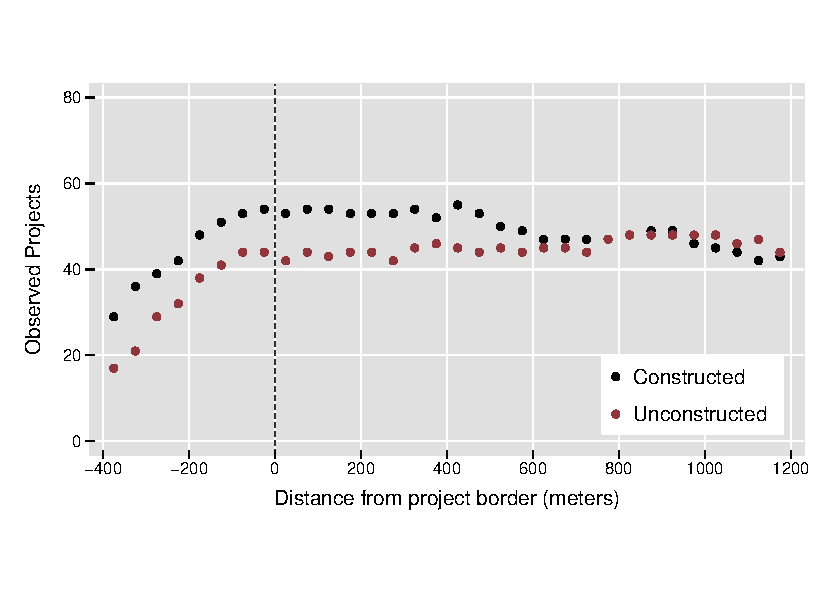
\includegraphics[scale=1.2,trim={.2cm 1.2cm .2cm 1.2cm},clip]{figures/projectcounts.pdf}
\end{figure}

\end{document}


